\documentclass[a4paper, 11pt]{article}
\usepackage{graphicx} % Required for inserting images
\usepackage{parskip}
\usepackage[shortlabels]{enumitem}
\usepackage{geometry}
\usepackage{titling}
\usepackage{multirow}
\usepackage{verbatim}
\usepackage{array}
\usepackage{microtype}
\usepackage{changepage}
\usepackage{ragged2e}
\usepackage{longtable}
\geometry{margin=2cm}
\setlength{\arrayrulewidth}{0.5mm}
\setlength{\tabcolsep}{15pt}
\setcounter{secnumdepth}{0}
\renewcommand{\arraystretch}{1.5}
\let\newline\\



\title{GYST 5e}
\date{}
\author{}
\begin{document}
\setlength{\parskip}{6pt}
\setlength{\parindent}{12pt}
\setlist[itemize]{leftmargin=*}
\setlist[enumerate]{leftmargin=*}
\maketitle

\begin{flushright}
\textbf{Membri del team di sviluppo:}
\\Valentina Bacchelli 1021155
\\Francesco Bufalini 1028917
\end{flushright}

\renewcommand\contentsname{Sommario}

\newpage
\tableofcontents



\newpage
\section{Abstract}
Questo progetto propone il design di un'applicazione dedicata alla creazione e gestione di creature nel contesto del gioco di ruolo Dungeons \& Dragons 5e. Il software mira a fornire agli utenti un ambiente intuitivo per modellare le creature controllate dai giocatori e/o le loro opzioni di personalizzazione.
Inoltre si vogliono ridurre le interruzioni del flusso di gioco automatizzando i calcoli matematici richiesti ai giocatori durante lo svolgimento e basati sulle opzioni possedute dalle loro creature. 



\newpage
\section{Analisi dei requisiti}
\subsection{Requisiti del sistema}

\begin{itemize}
    \item Per giocare, un utente crea delle Creature attraverso le Voci nel suo Compendio come definite nel Vocabolario.
    \item L’Utente può:
    \begin{itemize}
        \item visualizzare e modificare le Voci del proprio Compendio
        \item creare voci nel proprio Compendio, definendo i privilegi, le statistiche e i modificatori a essa associati
        \item importare Voci da un Compendio esterno o esportarne dal proprio
        \item creare e modificare Creature facendogli prendere o rimuovendo Voci del Compendio
        \item effettuare Riposi Brevi o Lunghi in qualsiasi momento per ripristinare le risorse delle Creature
        \item gestire i Privilegi delle Voci, selezionando quali privilegi prendere quando viene acquisita una Voce o quando si effettua il riposo dichiarato nella Voce
        \item modificare la quantità di un Oggetto posseduto da una Creatura e il livello di una Classe posseduta da una Creatura
        \item visualizzare le statistiche della creatura come formula o come numero (il risultato della formula), a cui vengono applicati automaticamente i modificatori attivi
        \item far subire danni di un certo tipo alla creatura, a cui vengono applicati automaticamente i modificatori attivi
        \item visualizzare i Modificatori posseduti dalle sue creature e quali sono attivi
        \item attivare e disattivare i Modificatori delle sue creature
    \end{itemize}
\end{itemize}


\newcounter{rf}
\newcommand\rf{\stepcounter{rf}\therf}
\newcounter{rnf}
\newcommand\rnf{\stepcounter{rnf}\thernf}
\newpage
\subsubsection{Tabella dei requisiti}

\begin{center}
    \begin{longtable}{ |l|p{10cm}|l|  }
        \hline
        \textbf{ID} & \textbf{REQUISITO} & \textbf{TIPO} \\ 
        \hline
        R\rf F & L’applicazione deve permettere di aggiungere, modificare, rimuovere e visualizzare le Voci del Compendio definite in un Manuale & Funzionale \\\hline
        R\rf F & L’applicazione deve permettere di esportare una Voce dal proprio Compendio o importarne di esterne & Funzionale \\\hline
        R\rf F & L’applicazione deve permettere di creare, modificare,\newline eliminare, duplicare e visualizzare le Creature possedute & Funzionale \\\hline
        R\rf F & L’applicazione deve permettere di importare ed esportare Creature  & Funzionale \\\hline
        R\rf F & L’applicazione deve permettere di selezionare, per ogni Creatura, le Voci possedute da quelle nel compendio & Funzionale \\\hline
        R\rf F & L’applicazione deve permettere, per ogni Creatura, di effettuare un Riposo Breve o un Riposo Lungo in qualsiasi momento & Funzionale \\\hline
        R\rf F & L’applicazione deve permettere, per ogni Creatura, di effettuare la selezione dei Privilegi della Voce che si vogliono possedere quando viene presa una Voce o quando viene effettuato il riposo dichiarato nella Voce & Funzionale \\\hline
        R\rf F & L’applicazione deve permette di definire, visualizzare e\newline modificare Formule Matematiche che possono includere delle variabili e l’equivalente di un lancio di dado & Funzionale \\\hline
        R\rf F & L’applicazione deve permettere di aggiungere, modificare, rimuovere e visualizzare Statistiche e Modificatori all’interno di una Voce del Compendio o di una Creatura & Funzionale \\\hline
        R\rf F & L’applicazione deve permettere di identificare ogni Formula Matematica definita da una Statistica in modo univoco e gerarchico, in modo che si possano applicare Modificatori alle singole Formule o a gruppi logici di esse & Funzionale \\\hline
        R\rf F & L’applicazione deve calcolare, per ogni Formula mostrata in una Creatura, il risultato numerico della formula, esclusi i lanci di dado che vanno lasciati come operazione sotto forma di stringa, e mostrarlo insieme ai pezzi della Formula non calcolati & Funzionale \\\hline
        R\rf F & L’applicazione deve mostrare, per ogni Creatura, i Modificatori posseduti dalla Creatura e quali di questi sono attivi & Funzionale \\\hline
        R\rf F & L’applicazione deve permettere, per ogni Creatura, di attivare o disattivare i modificatori posseduti & Funzionale \\\hline
        R\rf F & L’applicazione deve mostrare, per ogni Creatura, le Statistiche possedute e la Formula di ognuna dopo aver applicato i Modificatori che la bersagliano e aver calcolato il risultato secondo le Statistiche dela Creatura & Funzionale \\\hline
        R\rf F & L’applicazione deve permettere di cambiare il livello di una Classe posseduta da una Creatura & Funzionale \\\hline
        R\rf F & L’applicazione deve permettere di cambiare la quantità di un Oggetto posseduto da una creatura & Funzionale \\\hline
        R\rf F & L’applicazione deve permettere, per ogni Creatura, di Subire Danni, cioè inserire un intero e un Tipo di Danno e sottrarre l’intero ai Punti Ferita della creatura dopo aver applicato i modificatori per quel Tipo Di Danno & Funzionale \\\hline
        R\rf F & L’applicazione deve assicurarsi che ogni creatura presenti le Statistiche e i Modificatori di Base comuni a tutte le Creature & Funzionale \\\hline
        R\rnf NF & Una Voce del Compendio non può essere presa due volte dalla stessa Creatura & Non Funzionale \\\hline
        R\rnf NF & Il Livello Totale di una Creatura deve essere sempre la somma dei livelli delle sue Classi & Non Funzionale \\\hline        
        R\rnf NF & Ogni Voce posseduta dalla Creatura deve essere presente nel Compendio & Non Funzionale \\\hline
        R\rnf NF & All'importazione di una Creatura le Voci che possiede devono essere aggiunte al Compendio se non sono già presenti e in caso di incompatibilità questa va segnalata & Non Funzionale \\\hline      
        R\rnf NF & Quando viene esportata una Creatura vengono esportate anche le Voci del Compendio che possiede & Non Funzionale \\\hline
        R\rnf NF & Non possono essere definite due Statistiche con lo stesso identificatore & Non Funzionale \\\hline
        R\rnf NF & Non possono essere definiti due modificatori con lo stesso nome & Non Funzionale \\\hline        
        R\rnf NF & Non possono essere definite due Voci con lo stesso nome nello stesso manuale & Non Funzionale \\\hline        
        R\rnf NF & Una Formula Matematica definita da una Statistica deve essere identificabile tramite il nome della Statistica o il Tipo di Tiro (se presenta lanci di dado) & Non Funzionale \\\hline        
        R\rnf NF & Una Formula Matematica deve presentare solo variabili con nome di Statistiche già definite nel Compendio e non può referenziare se stessa & Non Funzionale \\\hline        
        R\rnf NF & Una Formula Matematica usata da una Creatura deve presentare solo variabili con nome di Statistiche già definite dalle voci possedute dalla Creatura e non può referenziare se stessa & Non Funzionale \\\hline    
        R\rnf NF & Una Formula Matematica deve essere in un formato che restituisca un singolo intero se si eseguono i tiri di dado e le operazioni matematiche che contiene & Non Funzionale \\\hline        
        R\rnf NF & Quando si applicano i Modificatori a una Formula e si mostra la Formula risultante vanno mostrati tutti i Modificatori applicati & Non Funzionale \\\hline        
        R\rnf NF & Devono poter esistere creature duplicate & Non Funzionale \\\hline        
        R\rnf NF & Una creatura deve possedere ogni voce del compendio secondo le quantità descritte nel vocabolario & Non Funzionale \\\hline        
        R\rnf NF & Non si possono modificare le Statistiche e i Modificatori di Base & Non Funzionale \\\hline   
        R\rnf NF & Nella schermata relativa a una Creatura, si devono mostrare all'utente tutte e solo le Statistiche definite come necessarie dalle Voci del Compendio possedute e dalla Creatura stessa& Non Funzionale \\\hline
        R\rnf NF & I danni subiti devono sempre essere positivi & Non Funzionale \\\hline        
        R\rnf NF & Velocità di memorizzazione dei dati & Non Funzionale \\\hline        
        R\rnf NF & Semplicità di navigazione nell’applicazione & Non Funzionale \\\hline        
        R\rnf NF & Ottimizzazione del tempo di aggiornamento delle interfacce al cambiamento di stato & Non Funzionale \\\hline
        R\rnf NF & Facile manutenibilità ed estensione futura & Non Funzionale \\\hline
    \end{longtable}
\end{center}



\newpage
\subsection{Analisi del dominio}
\subsubsection{Glossario}
\begin{center}
\setlength\LTleft{-1cm}
\setlength\LTright{-1cm}
    \begin{longtable}{ |p{3.5cm}|p{9cm}|p{3cm}|  }
        \hline
        \textbf{VOCE} & \textbf{DEFINIZIONE} & \textbf{SINONIMI} \\
        \hline
        Dungeons \& Dragons & Un gioco di ruolo dove i giocatori controllano e interpretano le azioni delle loro Creature per sviluppare una storia. È diviso in edizioni e la quinta è quella interessata dall’applicazione, che tuttavia tratterà solo una sottoparte del gioco, come indicato nell'abstract.  & D\&D, DnD \\
        \hline
        Giocatore & L'utente che usa l'applicazione. & \\\hline
        Compendio & Una serie di Voci del Compendio divise in base al Manuale che le definisce. È la lista da cui il giocatore sceglie le Voci per personalizzare la sua Creatura. & \\\hline
        Manuale & Un gruppo di Voci del Compendio con un nome, nella realtà rappresenta un libro pubblicato dagli autori del gioco come espansione. & \\\hline
        Voce del Compendio & Un’opzione di personalizzazione per le Creature, identificata da un nome e una descrizione. Durante la Creazione della Creatura e nel corso del gioco, le Voci possono essere prese o rimosse dalla Creatura. Le Voci definiscono tratti della Creatura e possono includere Statistiche e Modificatori. In una voce possono essere dichiarate delle Statistiche (definite da altre Voci o Creature) che vanno mostrate nella schermata di una Creatura quando questa possiede la Voce. Ogni Voce può avere sotto-voci (Privilegi), tra cui la Creatura può selezionare una certa quantità, e la scelta può ripetersi in particolari condizioni (vedi Riposo). Le Voci sono inoltre categorizzate per tipo, limitando il numero di Voci dello stesso tipo che una Creatura può avere. & Voce \\\hline
        Razza & Tipo di Voce del Compendio.  Se ne possiede sempre una e solo una, scelta alla creazione del Personaggio e modificata eventualmente in seguito. & \\\hline
        Classe & Tipo di Voce del Compendio. Alla creazione, e ogni altra volta che aumenta il Livello della Creatura, essa sceglie una Classe in cui prendere il Livello, ciò avviene aumentando il relativo Livello di Classe per quella Creatura. Il Livello di Classe all’inizio è 0 per ogni Classe. Il Livello di una Creatura sarà calcolabile dalla somma dei Livelli che ha preso in ogni Classe. Prendere un livello in una Classe aumenta il massimo dei Punti Ferita (vedi Statistiche Base in Creatura) di un numero dipendente dalla Classe. & \\\hline
        Background & Tipo di Voce del Compendio. Ne può essere scelto uno alla creazione del Personaggio. & \\\hline
        Talento &  Tipo di Voce del Compendio. Può essere concesso a una Creatura in accordo con gli altri Giocatori. & \\\hline
        Oggetto & Tipo di Voce del Compendio. Gli Oggetti definiti nel Compendio possono essere aggiunti o tolti agli Inventari delle Creature secondo lo svolgimento del gioco, in quantità variabili. È identificato da un Tipo di Oggetto. & \\\hline
         Tipo di Oggetto & Un attributo degli Oggetti. Può avere un supertipo, appartenere a un Tipo significa appartenere anche a tutti i suoi supertipi. A un Tiro di Dadi può essere associato un Oggetto che si usa per il Tiro, in questo modo vi si possono applicare dei Modificatori ai Tiri basati nello specifico su quell’Oggetto o sul suo Tipo. & \\\hline
         Privilegio & Tipo di Voce del Compendio usata per rappresentare le sotto-voci. Se ne ottengono selezionandone un numero quando si prende la Voce Del Compendio che li definisce oppure alla fine di un Riposo. Un Privilegio ha, come le altre Voci, un nome, una descrizione e dei sotto-privilegi. & \\\hline
         Formula Matematica & Le Formule Matematiche del gioco sono composte da una combinazione di stringhe che rappresenta nomi di Statistiche utilizzate come variabili, lanci di dado, numeri e operatori matematici. Ogni Formula può avere un valore massimo e/o un valore minimo. Ogni Formula è in un formato tale che se vengono sostituite le variabili ed effettuati i lanci di dado si ottiene una formula numerico/matematica che restituisce un risultato se calcolata. L'applicazione effettuerà tutte le operazioni fra interi quando verrà visualizzata la Formula nel contensto di una Creatura (quindi usando le sue Statistiche come variabili), tranne i lanci di dado. Questo porta a un risultato intero se non ci sono lanci di dado, oppure a una Formula composta solo da lanci di dado operati tra di loro e con un singolo intero. Quando si calcola il risultato, se la Formula non include lanci di dadi, il risultato viene portato al massimo se supera il valore massimo, o al minimo se non raggiunge quest’ultimo. & Formula \\\hline
         Tiro di Dadi & Il gioco può dichiarare che il risultato di una certa azione è determinato lanciando certi dadi e operando matematicamente sui risultati dei lanci  e i valori delle Statistiche della creatura per ottenere un intero (vedi Formula Matematica). Si rappresenta il dado lanciato con la formula d[numero di facce del dado], per esempio d6 per un dado a 6 facce (set corrispondente: {1, 2, 3, 4, 5, 6}), e si può aggiungere la quantità di dadi prima della ‘d’ per indicare che vanno lanciati più dadi uguali e i risultati sommati, per esempio la formula 2d6 corrisponde al lancio di due dadi a 6 facce con conseguente somma dei risultati. L’applicazione non si occupa di simulare i Tiri di Dadi. & Lancio di Dadi, Tiro \\\hline
         Statistica & Entità identificabile con un nome o Tipo di Tiro associata a una Formula Matematica, che definisce il suo valore per ogni Creatura. Una Statistica può avere una singola formula o una serie di formule, ognuna legata a un numero intero e a una Statistica di riferimento. Se la Formula ha un nome, può essere usata come variabile in altre Formule. Le Statistiche possono essere modificate da Modificatori specifici (per nome o Tipo di Tiro) o manualmente dal Giocatore. Una Statistica appartiene a una Creatura se definita da una Voce che questa possiede o se è inclusa nelle Statistiche Base per tutte le Creature (vedi Statistiche Base). Una Statistica può avere diverse "varianti" in base ai suoi attributi (oggetto usato in un tiro, caratterisitca usata in un tiro), quindi quando si dichiara un Modificatore si dice anche per quali attributi della statistica la bersaglia (tiri per colpire solo quando usano un certo oggetto per esempio), allo stesso modo una Voce può dichiarare una certa variante di una Statistica che va mostrata quando si possiede la voce& Stat\\\hline
         Caratteristiche & Nel gioco rappresentano le facoltà fisiche e mentali in cui una Creatura si può migliorare e che può usare per compiere un’azione. & \\\hline
         Forza & Caratteristica che rappresenta la potenza fisica. & \\\hline
         Destrezza & Caratteristica che rappresenta l'agilità.&\\\hline
         Costituzione & Caratteristica che rappresenta la resistenza. &\\\hline
         Intelligenza & Caratteristica che rappresenta il ragionamento e la memoria. &\\\hline
         Saggezza & Caratteristica che rappresenta la percezione e l'intuizione. &\\\hline
         Carisma & Caratteristica che rappresenta la forza di personalità.&\\\hline
         Punteggio \newline Caratteristica & Statistica Base delle Creature (vedi Statistiche di Base). Un intero positivo arbitrario, associato a una Caratteristica, concordato fra i giocatori e passato dall’utente, massimo 20 a meno che non ci siano Modificatori che dicano diversamente. & \\\hline
         Modificatore \newline Caratteristica & Statistica Base delle Creature (vedi Statistiche di Base). Non bisogna confondere la Statistica con questo nome con il concetto di Modificatori nonostante la somiglianza nel nome (vedi Modificatori). Il valore di questa statistica è un intero proporzionale al Punteggio Caratteristica associato alla stessa  Caratteristica, ottenibile sottraendovi 10 e dividendolo per 2, approssimando poi il risultato per difetto. & \\\hline
         Tipo di Tiro & Per identificare una Formula che contiene Lanci di Dadi al suo interno invece che il nome si usa un Tipo di Tiro. I Tipi di Tiro sono diversi, organizzati in una gerarchia, e ognuno presenta degli attributi. Un Modificatore può bersagliare più Statistiche con Tipo di Tiro indicando il valore richiesto da alcuni o nessuno dei suoi attributi (verranno bersagliate tutte le Formule che presentano un Tipo di Tiro che rispetta il vincolo sugli attributi). & \\\hline
        Tiro di d20 Base & Tipo di Tiro. La Formula identificata dal Tiro è fissa e pari a “d20” (estrazione di numero da 1 a 20) e non è modificabile dall’utente. Questi Tiri sono definiti nelle Statistiche Base e bersagliati dai modificatori. & \\\hline
        Tiro Caratteristica & Tipo di Tiro di d20 Base. Rappresenta un'azione di un personaggio in un certo campo. Quando si vuole effettuare un Tiro di questo tipo si sceglie sempre una Caratteristica associata e si può aggiungere o meno un'Abilità. & Prova Caratteristica, Tiro Abilità \\\hline
        Abilità & Nel mondo di gioco rappresentano aree di competenza più specifiche delle Caratteristiche.  Nella pratica, quando una Creatura fa una Prova Caratteristica può selezionare un Abilità che rappresenta l’azione (concordata fra i giocatori). Ogni Abilità è associata a una delle sei Caratteristiche e viene solitamente usata nelle Prove Caratteristica basate sulla Caratteristica associata, a meno che non venga specificato diversamente. & \\\hline
        Iniziativa & Abilità basata su Destrezza & \\\hline
        Acrobazia & Abilità basata su Destrezza & \\\hline
        Addestrare Animali & Abilità basata su Saggezza &   \\\hline
        Arcano & Abilità basata su Intelligenza & \\\hline
        Atletica &Abilità basata su Forza&\\\hline
        Furtività & Abilità basata su Destrezza & \\\hline
        Indagare & Abilità basata su Intelligenza & \\\hline
    Inganno & Abilità basata su Carisma & \\\hline
    Intimidire & Abilità basata su Carisma & \\\hline
    Intrattenere & Abilità basata su Carisma & \\\hline
    Natura & Abilità basata su Intelligenza & \\\hline
    Medicina &Abilità basata su Saggezza & \\\hline
    Intuire &Abilità basata su Saggezza & \\\hline
    Percezione &Abilità basata su Saggezza & \\\hline
    Persuasione & Abilità basata su Carisma & \\\hline
    Rapidità di Mano & Abilità basata su Destrezza & \\\hline
    Religione & Abilità basata su Intelligenza & \\\hline
    Sopravvivenza & Abilità basata su Saggezza & \\\hline
    Storia & Abilità basata su Intelligenza & \\\hline
    Prova di Lotta & Un Tiro Caratteristica su Atletica può essere o no una Prova di Lotta, che rappresenta una contesa con un'altra Creatura in battaglia. & \\\hline
    Tiro per Colpire & Tipo di Tiro di d20 Base. Rappresenta l’azione di cercare di colpire un’altra Creatura. Il suo unico attributo è il Tipo di Attacco. & TxC \\\hline
    Tipo di Attacco & Usato per rappresentare Azioni Offensive, va sempre dichiarato nei Tiri per Colpire. Si divide in Attacco in Mischia, per azioni su Creature vicine, e Attacco a Distanza, per azioni su Creature distanti. & \\\hline
    Tiro Salvezza & Tipo di Tiro di d20 Base. Rappresenta l’azione di cercare di evitare o minimizzare un effetto negativo. Si basa quasi sempre su una Caratteristica. & \\\hline
    Tiro con nome & Una formula con lanci di dado e un nome a identificarla & \\\hline
    Tiro per i Danni & Tipo di Tiro con nome. Un tiro per valutare l’entità di danni fatti alle altre creature a seguito di un’evento nel gioco. Può essere definito in una Voce del Compendio e i dadi lanciati e le operazioni che vi vengono compiute sono dichiarati staticamente in forma di Formula nella Voce . Ha sempre un Tipo di Danno associato usato nei vincoli dei Modificatori per specificare se si applicano o no al Tiro. & \\\hline
    Tipo di Danno & Ogni volta che si fa un Tiro per i Danni o si Subiscono Danni, a rappresentare attraverso/da cosa si ferisce/viene feriti, bisogna dichiarare se il danno è magico e scegliere il Tipo di Danno. & \\\hline
    Acido & Tipo di Danno & \\\hline
    Contundente & Tipo di Danno & \\\hline
    Forza & Tipo di Danno & \\\hline
    Freddo & Tipo di Danno & \\\hline
    Fulmine & Tipo di Danno & \\\hline
    Fuoco & Tipo di Danno & \\\hline
    Necrotico & Tipo di Danno & \\\hline
    Psichico & Tipo di Danno & \\\hline
    Perforante & Tipo di Danno & \\\hline
    Radiante & Tipo di Danno & \\\hline
    Tagliente & Tipo di Danno & \\\hline
    Tuono & Tipo di Danno & \\\hline
    Veleno & Tipo di Danno & \\\hline
    Modificatore & I Modificatori rappresentano delle condizioni in cui si può trovare una Creatura che ha una certa Voce del Compendio. Sono definiti nella Voce o presenti nelle opzioni di Base della Creatura e specificano come identificare le Statistiche a cui si applicano quando attivi attraverso il nome della Statistica bersagliata o il suo Tipo di Tiro, oppure quando si applicano ai Danni Subiti attraverso il Tipo di Danno bersagliato. Nel modificatore è specificato come viene alterata la Formula bersagliata. & \\\hline
    Modificatori non cumulabili & Modificatori predefiniti che vengono applicati una volta sola anche se la Creatura ne ha altri dello steso tipo attivi sulla stessa Formula &\\\hline
    Competenza & Modificatore non cumulabile. Un tipo di Modificatore che può essere dato solo ai Tiri di d20 Base. Se una Creatura ne ha almeno uno attivo che si applica al Tiro che sta effettuando allora somma il suo Bonus Competenza (vedi Statistiche Base in Creatura) al risultato del Tiro. & \\\hline
    Maestria & Modificatore non cumulabile. Un tipo di Modificatore che viene dato solo ai Tiri di d20 Base su cui si ha già Competenza. Se una Creatura ne ha almeno uno attivo che si applica al Tiro che sta effettuando allora somma di nuovo il suo Bonus Competenza (vedi Statistiche Base in Creatura) al risultato del Tiro. & \\\hline
    Resistenza ai Danni & Modificatore non cumulabile. Quando una Creatura ha almeno una Resistenza attiva su un Tipo di Danno e subisce Danni di quel tipo dimezza e arrotonda per difetto i Danni prima di applicarli. & \\\hline
    Vulnerabilità ai Danni & Modificatore non cumulabile. Quando una Creatura ha almeno una Vulnerabilità attiva su un Tipo di Danno e subisce Danni di quel tipo duplica i Danni prima di applicarli. & \\\hline
    Immunità ai Danni & Modificatore non cumulabile. Quando una Creatura ha almeno un’Immunità attiva su un Tipo di Danno e subisce Danni di quel tipo azzera i Danni prima di applicarli. & \\\hline
    Creatura & Un entità controllata dal giocatore a cui appartiene che ne descrive le azioni agli altri giocatori. & Entità, \newline Personaggio \\\hline
    Allineamento & Rappresenta la morale di una certa Creatura. Per ogni Creatura va scelto se è Caotico, Neutrale o Legale poi se è Malvagio, Neutrale o Buono. L’Allineamento è la combinazione di queste due scelte e può cambiare nel tempo. & \\\hline
    Statistiche di Base & Statistiche comuni a tutte le Creature e non associate a una Voce. & \\\hline
    Livello della Creatura & Statistica Base che parte da 1 alla creazione e aumenta quando si prende un livello in una Classe. & Livello Totale, Livello \\\hline
    Livello di Classe & Statistica Base per ogni Classe presentata dalla Creatura. Rappresenta il numero di volte che la Creatura ha preso quella Classe. & \\\hline
    Bonus Competenza & Statistica Base che parte da 2 e aumenta quando si raggiungono certi Livelli della Creatura. & \\\hline
    Punti Ferita & Statistica Base che che rappresenta la salute di una creatura, ritorna al suo massimo dopo ogni Riposo Lungo e non scende mai sotto lo 0. Quando si subiscono Danni questi vengono detratti prima ai Punti Ferita Temporanei poi ai Punti Ferita. & PF \\\hline
    Punti Ferita Temporanei & Statistica Base. Un numero positivo normalmente a 0 che può essere aumentato dai Privilegi. Quando si Subiscono Danni vengono prima scalati i Punti Ferita Temporanei e poi, se ne avanzano, si detrae il resto dai Punti Ferita Attuali. & PF Temporanei \\\hline
    Classe Armatura & Statistica Base che contiene un numero positivo, è inizialmente pari a 10+Modificatore di Destrezza. Quando un giocatore fa un Tiro per Colpire a una Creatura il proprietario della Creatura bersaglio dovrà dichiarare la sua CA che sarà confrontata col risultato del Tiro. & CA \\\hline
    Velocità & Statistica Base che indica quanto veloce è in una Creatura a muoversi in un certo modo. Si suddivide in 6 tipi di Velocità. Se non modificato da un Modificatore, il valore predefinito della velocità dipende dal tipo. Esso è pari a 0 per i primi tre tipi di Velocità dell’elenco e pari a Velocità di Movimento diviso due (arrotondata per difetto) per gli ultimi tre. & \\\hline
    Velocità di \newline Movimento& Tipo di Velocità & \\\hline
    Velocità di Volo& Tipo di Velocità & \\\hline
    Velocità di Scavo& Tipo di Velocità & \\\hline
    Velocità di Nuoto& Tipo di Velocità & \\\hline
    Velocità di \newline Arrampicata& Tipo di Velocità & \\\hline
    Velocità Furtiva& Tipo di Velocità & \\\hline
    Modificatori di Base & Modificatori comuni a tutte le Creature. & \\\hline
    Riposo & Nel gioco, rappresenta l'azione di riposarsi. Consente di ripetere la scelta dei Privilegi per alcune Voci del Compendio e di ripristinare certe Statistiche al loro valore massimo o minimo. Si distingue in due tipi, in base alla durata. & \\\hline
    Riposo Breve & Tipo di Riposo & \\\hline
    Riposo Lungo & Tipo di Riposo & \\\hline
    \end{longtable}
\end{center}



\newpage
\subsection{Analisi dei requisiti}
\subsubsection{Casi d'uso}
\begin{figure}[h!]
    \centering
    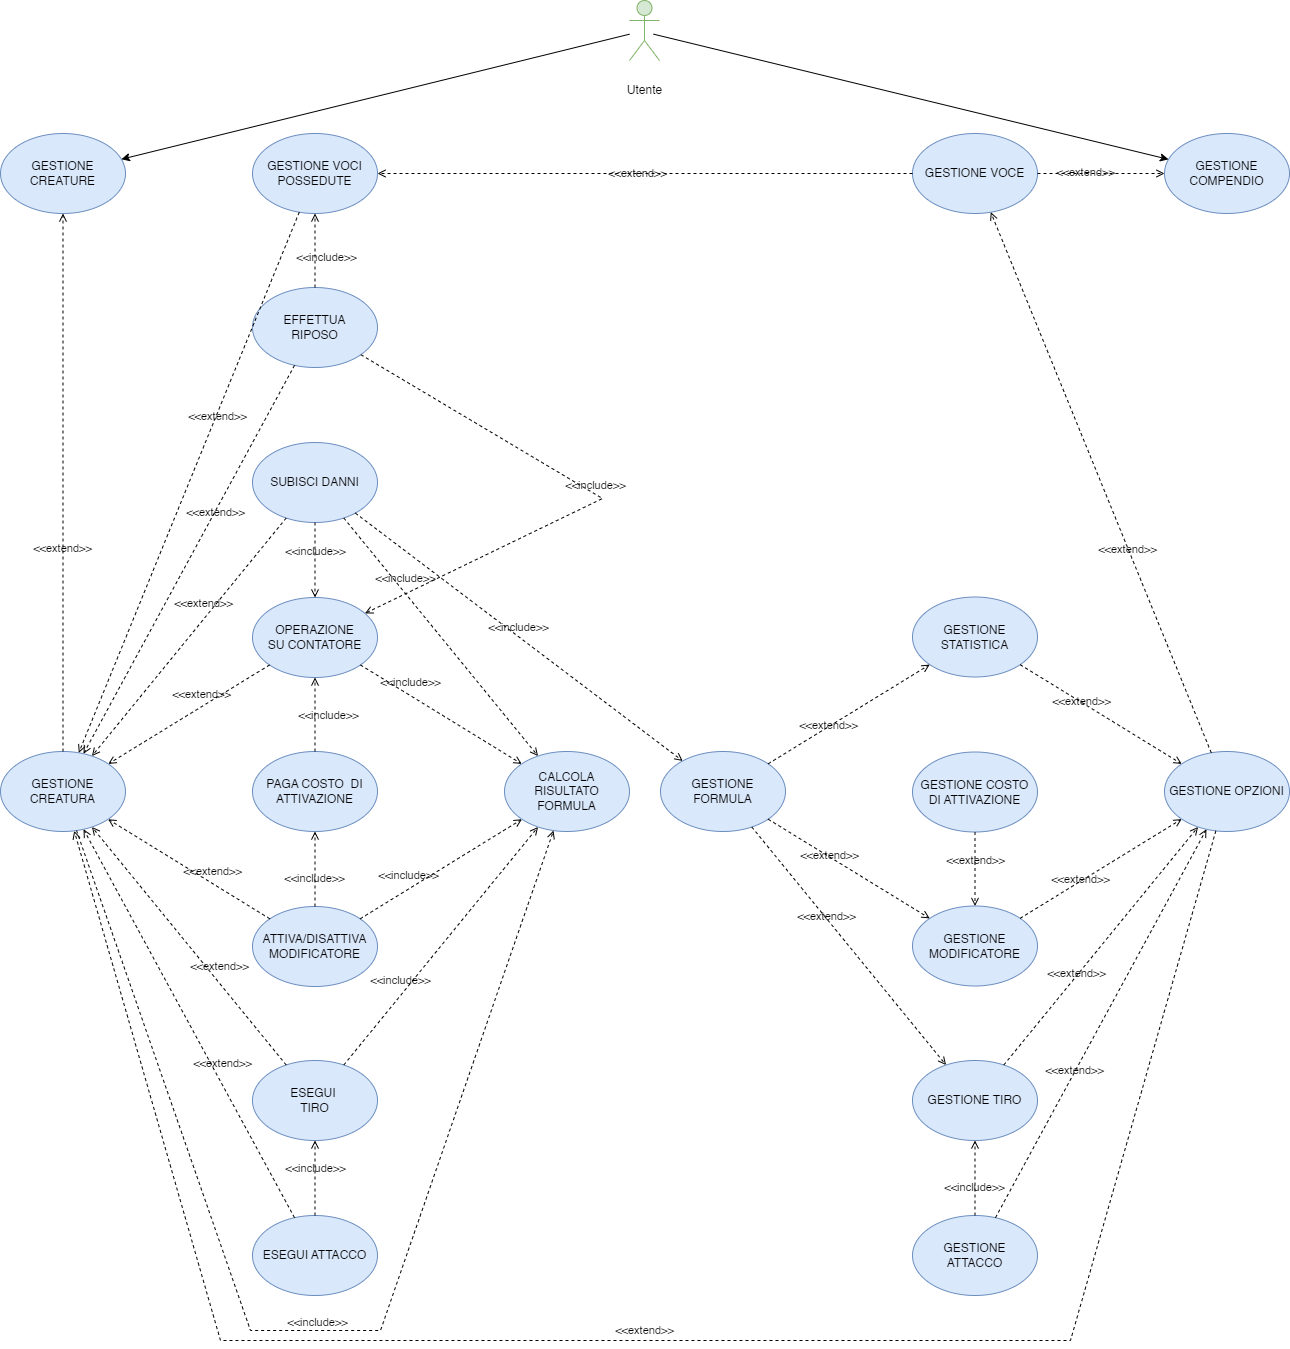
\includegraphics[width=1\textwidth,keepaspectratio]{Diagramma CU}
    \label{fig:useCase}
\end{figure}



\newpage
\subsubsection{Scenari}
\begin{center}

\begin{tabular}{ |p{5cm}|p{9.5cm}|  }
\hline
\textbf{Titolo} & Gestione Compendio \\
\hline
\textbf{Descrizione} & L'Utente visualizza e modifica le voci del suo compendio \\
\hline
\textbf{Attori} & Utente  \\
\hline
\textbf{Relazioni} & Gestione Voce \\
\hline
\textbf{Precondizioni} &  \\
\hline
\textbf{Postcondizioni} & Compendio aggiornato con le modifiche apportate \\
\hline
\textbf{Scenario principale} & 
\begin{enumerate}
    \item L'Utente seleziona la sezione di gestione del compendio
    \item Il Sistema mostra l'elenco di Voci del Compendio disponibili, divise per manuali
    \item L'Utente può visualizzarle, modificarle, aggiungerle, eliminarle, esportarle o importarne di nuove
\end{enumerate}
\\
\hline
\textbf{Scenari alternativi} & \\
\hline
    \textbf{Requisiti non funzionali} & R3NF; R4NF; R8NF \\
\hline
\textbf{Punti aperti} &  \\
\hline
\end{tabular}

\vspace{3em}

\begin{tabular}{ |p{5cm}|p{9.5cm}|  }
\hline
\textbf{Titolo} & Gestione Voce \\
\hline
\textbf{Descrizione} & L'Utente visualizza una voce e ne cambia gli attributi \\
\hline
\textbf{Attori} & Utente  \\
\hline
\textbf{Relazioni} & Gestione Compendio; Gestione Statistica; Gestione Modificatore \\
\hline
\textbf{Precondizioni} &  \\
\hline
\textbf{Postcondizioni} & Voce aggiornata con le modifiche apportate \\
\hline
\textbf{Scenario principale} & 
\begin{enumerate}
    \item L'Utente sceglie una voce da una lista
    \item L'Utente la visualizza e può modificarla
\end{enumerate}
\\
\hline
\textbf{Scenari alternativi} & \\
\hline
    \textbf{Requisiti non funzionali} & R8NF \\
\hline
\textbf{Punti aperti} &  \\
\hline
\end{tabular}

\vspace{3em}


\begin{tabular}{ |p{5cm}|p{9.5cm}|  }
\hline
\textbf{Titolo} & Gestione Modificatore \\
\hline
\textbf{Descrizione} & L'Utente visualizza, crea o modifica un modificatore definito in una voce o in una creatura \\
\hline
\textbf{Attori} & Utente  \\
\hline
\textbf{Relazioni} & Gestione Voce, Gestione Formula \\
\hline
\textbf{Precondizioni} &  \\
\hline
\textbf{Postcondizioni} & Modificatore aggiornato con le modifiche apportate \\
\hline
\textbf{Scenario principale} & 
\begin{enumerate}
    \item L'Utente seleziona un modificatore o ne crea uno nuovo
    \item Lo visualizza e può cambiarne il nome, le formule a cui si applica, o la modifica che esso apporta quando applicato
\end{enumerate}
\\
\hline
\textbf{Scenari alternativi} &Il nome corrisponde a quello di un altro modificatore posseduto dalla creatura e ne viene richiesta la modifica \\
\hline
    \textbf{Requisiti non funzionali} &  R7NF; R13NF; R16NF \\
\hline
\textbf{Punti aperti} &  \\
\hline
\end{tabular}

\vspace{3em}

\begin{tabular}{ |p{5cm}|p{9.5cm}|  }
\hline
\textbf{Titolo} & Gestione Statistica \\
\hline
\textbf{Descrizione} & L'Utente visualizza, crea o modifica una Statistica \\
\hline
\textbf{Attori} & Utente  \\
\hline
\textbf{Relazioni} & Gestione Voce, Gestione Formula \\
\hline
\textbf{Precondizioni} &  \\
\hline
\textbf{Postcondizioni} & Statistica aggiornata con le modifiche apportate \\
\hline
\textbf{Scenario principale} & 
\begin{enumerate}
    \item L'Utente crea una Statistica o ne sceglie una
    \item La visualizza e può modificarla
\end{enumerate}
\\
\hline
\textbf{Scenari alternativi} &La formula definita dalla Statistica è invalida e quindi va modificata prima di uscire, oppure il nome o il Tipo di Tiro corrisponde a quello di un'altra opzione posseduta dalla creatura e ne viene richiesta la modifica \\
\hline
    \textbf{Requisiti non funzionali} & R6NF; R9NF; R16NF \\
\hline
\textbf{Punti aperti} &  \\
\hline
\end{tabular}

\vspace{3em}

\begin{tabular}{ |p{5cm}|p{9.5cm}|  }
\hline
\textbf{Titolo} & Gestione Formula \\
\hline
\textbf{Descrizione} & L'Utente visualizza, crea o modifica una Formula \\
\hline
\textbf{Attori} & Utente  \\
\hline
\textbf{Relazioni} & Gestione Statistica, Gestione Modificatore \\
\hline
\textbf{Precondizioni} &  \\
\hline
\textbf{Postcondizioni} & Formula aggiornata con le modifiche apportate e validata \\
\hline
\textbf{Scenario principale} & 
\begin{enumerate}
    \item L'Utente crea una Formula o ne sceglie una
    \item La visualizza e può modificarla
\end{enumerate}
\\
\hline
\textbf{Scenari alternativi} &La formula è invalida e quindi va modificata prima di uscire \\
\hline
    \textbf{Requisiti non funzionali} & R9NF; R10NF; R11NF; R12NF; R13NF\\
\hline
\textbf{Punti aperti} &  \\
\hline
\end{tabular}

\vspace{3em}

\begin{tabular}{ |p{5cm}|p{9.5cm}|  }
\hline
\textbf{Titolo} & Gestione Creature \\
\hline
\textbf{Descrizione} & L'Utente visualizza e gestisce le creature nella sua lista \\
\hline
\textbf{Attori} & Utente  \\
\hline
\textbf{Relazioni} & Gestione Creatura\\
\hline
\textbf{Precondizioni} &  \\
\hline
\textbf{Postcondizioni} & Lista delle creature aggiornata \\
\hline
\textbf{Scenario principale} & L'Utente visualizza le creature disponibili e le gestisce secondo le sue esigenze potendo:
\begin{enumerate}
    \item Crearle
    \item Eliminarle
    \item Gestirle
    \item Duplicarle
    \item Importarle
    \item Esportarle
\end{enumerate} \\
\hline
\textbf{Scenari alternativi} & \\
\hline
\textbf{Requisiti non funzionali} & R4NF; R5NF; R14NF\\
\hline
\textbf{Punti aperti} & \\
\hline
\end{tabular}

\vspace{3em}

\begin{tabular}{ |p{5cm}|p{9.5cm}|  }
\hline
\textbf{Titolo} & Gestione Creatura \\
\hline
\textbf{Descrizione} & L'Utente gestisce una creatura fra quelle possedute \\
\hline
\textbf{Attori} & Utente \\
\hline
\textbf{Relazioni} & Gestione Creature; Gestione Voci Possedute; Effettua Riposo; Subisci Danni; Attiva/Disattiva Modificatore; Calcola Risultato Formula \\
\hline
\textbf{Precondizioni} & \\
\hline
\textbf{Postcondizioni} & Salvato nuovo stato della Creatura\\
\hline
\textbf{Scenario principale} & L'Utente entra nell'interfaccia di gestione di una creatura dove gli vengono mostrati:
\begin{enumerate}
    \item Le informazioni base della creatura (nome e allineamento)
    \item La sezione per gestire le sue voci possedute
    \item I modificatori posseduti dalla creatura e se sono attivi o no
\end{enumerate} \\
\hline
\textbf{Scenari alternativi} & \\
\hline
\textbf{Requisiti non funzionali} & R2NF, R17NF\\
\hline
\textbf{Punti aperti} &  \\
\hline
\end{tabular}

\vspace{3em}

\begin{tabular}{ |p{5cm}|p{9.5cm}|  }
\hline
\textbf{Titolo} & Gestione Voci Possedute \\
\hline
\textbf{Descrizione} & L'Utente visualizza e gestisce le voci del compendio possedute da una creatura \\
\hline
\textbf{Attori} & Utente \\
\hline
\textbf{Relazioni} & Gestione Creatura; Effettua Riposo \\
\hline
\textbf{Precondizioni} & Creatura rispetta vincoli su quante Voci del Compendio può possedere per ogni Tipo \\
\hline
\textbf{Postcondizioni} & Lista di voci possedute della creatura aggiornata \\
\hline
\textbf{Scenario principale} & 
\begin{enumerate}
    \item L'Utente accede alla sezione di gestione delle voci possedute
    \item L'Utente ha l'opzione di aggiungere voci, rimuoverle, sostituirle. In più da qui si scelgono i privilegi selezionati per ogni voce e si possono cambiare il livello di una classe o la quantità di un oggetto
\end{enumerate}\\
\hline
\textbf{Scenari alternativi} & \\
\hline
\textbf{Requisiti non funzionali} & R1NF; R3NF; R15NF\\
\hline
\textbf{Punti aperti} & \\
\hline
\end{tabular}

\vspace{3em}

\begin{tabular}{ |p{5cm}|p{9.5cm}|  }
\hline
\textbf{Titolo} & Effettua Riposo \\
\hline
\textbf{Descrizione} & La Creatura dell'Utente fa un riposo lungo o corto innescando la scelta dei privilegi e se è un riposo lungo recupera pf fino al loro valore massimo \\
\hline
\textbf{Attori} & Utente \\
\hline
\textbf{Relazioni} & Gestione Creatura; Gestione Voci Possedute \\
\hline
\textbf{Precondizioni} & \\
\hline
\textbf{Postcondizioni} & È stata rieffettuata la selezione dei privilegi che si ripetono al riposo e se il riposo è lungo i pf tornano al loro valore massimo\\
\hline
\textbf{Scenario principale} & 
\begin{enumerate}
    \item L'Utente dichiara di voler effettuare un riposo
    \item L'Utente seleziona il tipo di riposo che effettua
    \item Viene proposto di ripetere la selezione dei privilegi per le voci interessate al riposo
    \item Se il riposo è un riposo lungo, i pf vengono riportati al loro valore massimo
\end{enumerate}\\
\hline
\textbf{Scenari alternativi} & \\
\hline
\textbf{Requisiti non funzionali} & \\
\hline
\textbf{Punti aperti} & \\
\hline
\end{tabular}

\vspace{3em}

\begin{tabular}{ |p{5cm}|p{9.5cm}|  }
\hline
\textbf{Titolo} & Subisci Danni \\
\hline
\textbf{Descrizione} & L'Utente fa prendere danni alla creatura portando una riduzione dei suoi punti vita \\
\hline
\textbf{Attori} & Utente \\
\hline
\textbf{Relazioni} & Gestione Creatura; Calcola Risultato Formula \\
\hline
\textbf{Precondizioni} & \\
\hline
\textbf{Postcondizioni} & I punti vita della creatura vengono ridotti \\
\hline
\textbf{Scenario principale} & 
\begin{enumerate}
    \item L'Utente dichiara di voler prendere danni
    \item L'Utente seleziona il tipo di danno che prende
    \item L'Utente immette un intero che corrisponde ai danni presi
    \item L'applicazione controlla quali modificatori si applicano in base al tipo di danno
    \item L'Utente conferma i valori immessi
    \item Vengono applicati i modificatori attivi
    \item Viene sottratto il risultato dai Punti Ferita Attuali della Creatura
\end{enumerate}\\
\hline
\textbf{Scenari alternativi} & L'utente non conferma i danni e si ritorna all'interfaccia della gestione creatura\\
\hline
\textbf{Requisiti non funzionali} & R18NF \\
\hline
\textbf{Punti aperti} & \\
\hline
\end{tabular}

\vspace{3em}

\begin{tabular}{ |p{5cm}|p{9.5cm}|  }
\hline
\textbf{Titolo} & Attiva/Disattiva Modificatore \\
\hline
\textbf{Descrizione} & Viene invertito lo stato attuale di un modificatore\\
\hline
\textbf{Attori} & Utente \\
\hline
\textbf{Relazioni} & Gestione Creatura; Calcola Risultato Formula \\
\hline
\textbf{Precondizioni} & \\
\hline
\textbf{Postcondizioni} & Aggiornamento interfaccia gestione creatura e ricalcolo dei valori delle statistiche \\
\hline
\textbf{Scenario principale} & 
\begin{enumerate}
    \item L'Utente seleziona un modificatore posseduto da attivare o disattivare
    \item L'applicazione cambia lo stato del modificatore 
    \item L'applicazione mostra l'interfaccia di gestione della creatura aggiornata ricalcolando il valore per ogni statistica
\end{enumerate}\\
\hline
\textbf{Scenari alternativi} & \\
\hline
\textbf{Requisiti non funzionali} & R13NF\\
\hline
\textbf{Punti aperti} & \\
\hline
\end{tabular}

\vspace{3em}

\begin{tabular}{ |p{5cm}|p{9.5cm}|  }
\hline
\textbf{Titolo} & Calcola Risultato Formula \\
\hline
\textbf{Descrizione} & Viene scelta una formula di cui va calcolato il risultato, che viene restituito alla fine \\
\hline
\textbf{Attori} & Utente \\
\hline
\textbf{Relazioni} & Gestione Creatura; Subisci Danni; Attiva/Disattiva Modificatore \\
\hline
\textbf{Precondizioni} & La formula passata referenzia solo statistiche definite dalla creatura \\
\hline
\textbf{Postcondizioni} & \\
\hline
\textbf{Scenario principale} & 
\begin{enumerate}
    \item Vengono espanse le variabili (statistiche) usate nella formula
    \item Viene calcolato il risultato matematico della formula risultante, lasciando però eventuali tiri di dado contenuti in essa sotto forma di stringa nel formato "d[numero di facce del dado]", per esempio d6 per un dado a 6 facce
\end{enumerate}\\
\hline
\textbf{Scenari alternativi} &\\
\hline
\textbf{Requisiti non funzionali} & R12NF\\
\hline
\textbf{Punti aperti} & \\
\hline
\end{tabular}

\vspace{3em}

\end{center}

\newpage

\subsection{Analisi dei rischi}
\subsubsection*{Tabella Valutazione Beni}
\begin{center}
    \begin{tabular}{ |p{4cm}|p{5cm\RaggedRight}|p{4cm}|  }
        \hline
        \textbf{BENE} & \textbf{VALORE} & \textbf{ESPOSIZIONE} \\
        \hline
        Dati di Gioco & Medio. Lo scopo dell’applicazione è proprio gestirli. & Media. Compromissione dell’esperienza di gioco, perdita di progressi, dubbio sulla veridicità dei dati mostrati se attacco all’integrità dei dati. \\
        \hline
        Algoritmi e meccaniche di gioco & Medio. Proprietà intellettuale e interazione con il sistema a livello più basso. & Alta. Sfruttamento degli algoritmi per esecuzione di script malevoli (code injection). \\
        \hline
    \end{tabular}
\end{center}

\subsubsection*{Tabella Minacce e Controlli}
\begin{center}
    \begin{tabular}{|p{3cm}|p{3cm}|p{3cm}|p{3.5cm\RaggedRight}|}
        \hline
         \textbf{MINACCIA} & \textbf{PROBABILITÀ} & \textbf{CONTROLLO} & \textbf{FATTIBILITÀ} \\
         \hline
         Code Injection &Alta. Interpretazione di formule definite da altri utenti con possibili intenzioni malevole.& Sanitizzazione dell'input, utilizzo di prepared statements. & Medio costo. Richiede competenze di sviluppo sicuro, ma fondamentale per la sicurezza dell'app. \\
         \hline
         Modifiche non autorizzate dagli altri giocatori alle Creature & Media. Un giocatore potrebbe apportare modifiche alle proprie creature contro le regole del gioco all’insaputa degli altri. & Log condivisibile delle modifiche effettuate alle creature. & Basso costo. Già necessario per il rollback. \\
         \hline
         Perdita di dati & Media. Possibilità di perdita di dati critici del gioco. & Backup regolari, log delle azioni effettuate, procedure di rollback. & Medio costo. I sistemi di backup sono essenziali e spesso richiedono un investimento in hardware/software. \\
         \hline
         Ingiunzioni legali per contenuto non autorizzato & Media. Dipende dal rispetto dei diritti di proprietà intellettuale. & Filtraggio dei contenuti, politiche chiare. & Basso costo. Protezione legale e della reputazione. Sfruttamento dell’Open Game License. \\
         \hline
    \end{tabular}
\end{center}

\vspace{2em}

\subsubsection*{Analisi Tecnologica della Sicurezza}
\begin{center}
    \begin{tabular}{|p{6cm}|p{8cm}|}
        \hline
        \textbf{Tecnologia} & \textbf{Vulnerabilità} \\
        \hline
        Interprete di formule dinamiche & 
        \begin{itemize}
            \item Code Injection
        \end{itemize} \\
        
        \hline
        Log &
        \begin{itemize}
            \item Manipolazione e non integrità dei log
        \end{itemize}\\
        \hline 
    \end{tabular}
\end{center}



\newpage



\subsubsection{Security Use Case e Misuse Case}
\vspace{2em}
\begin{figure}[h!]
    \centering
    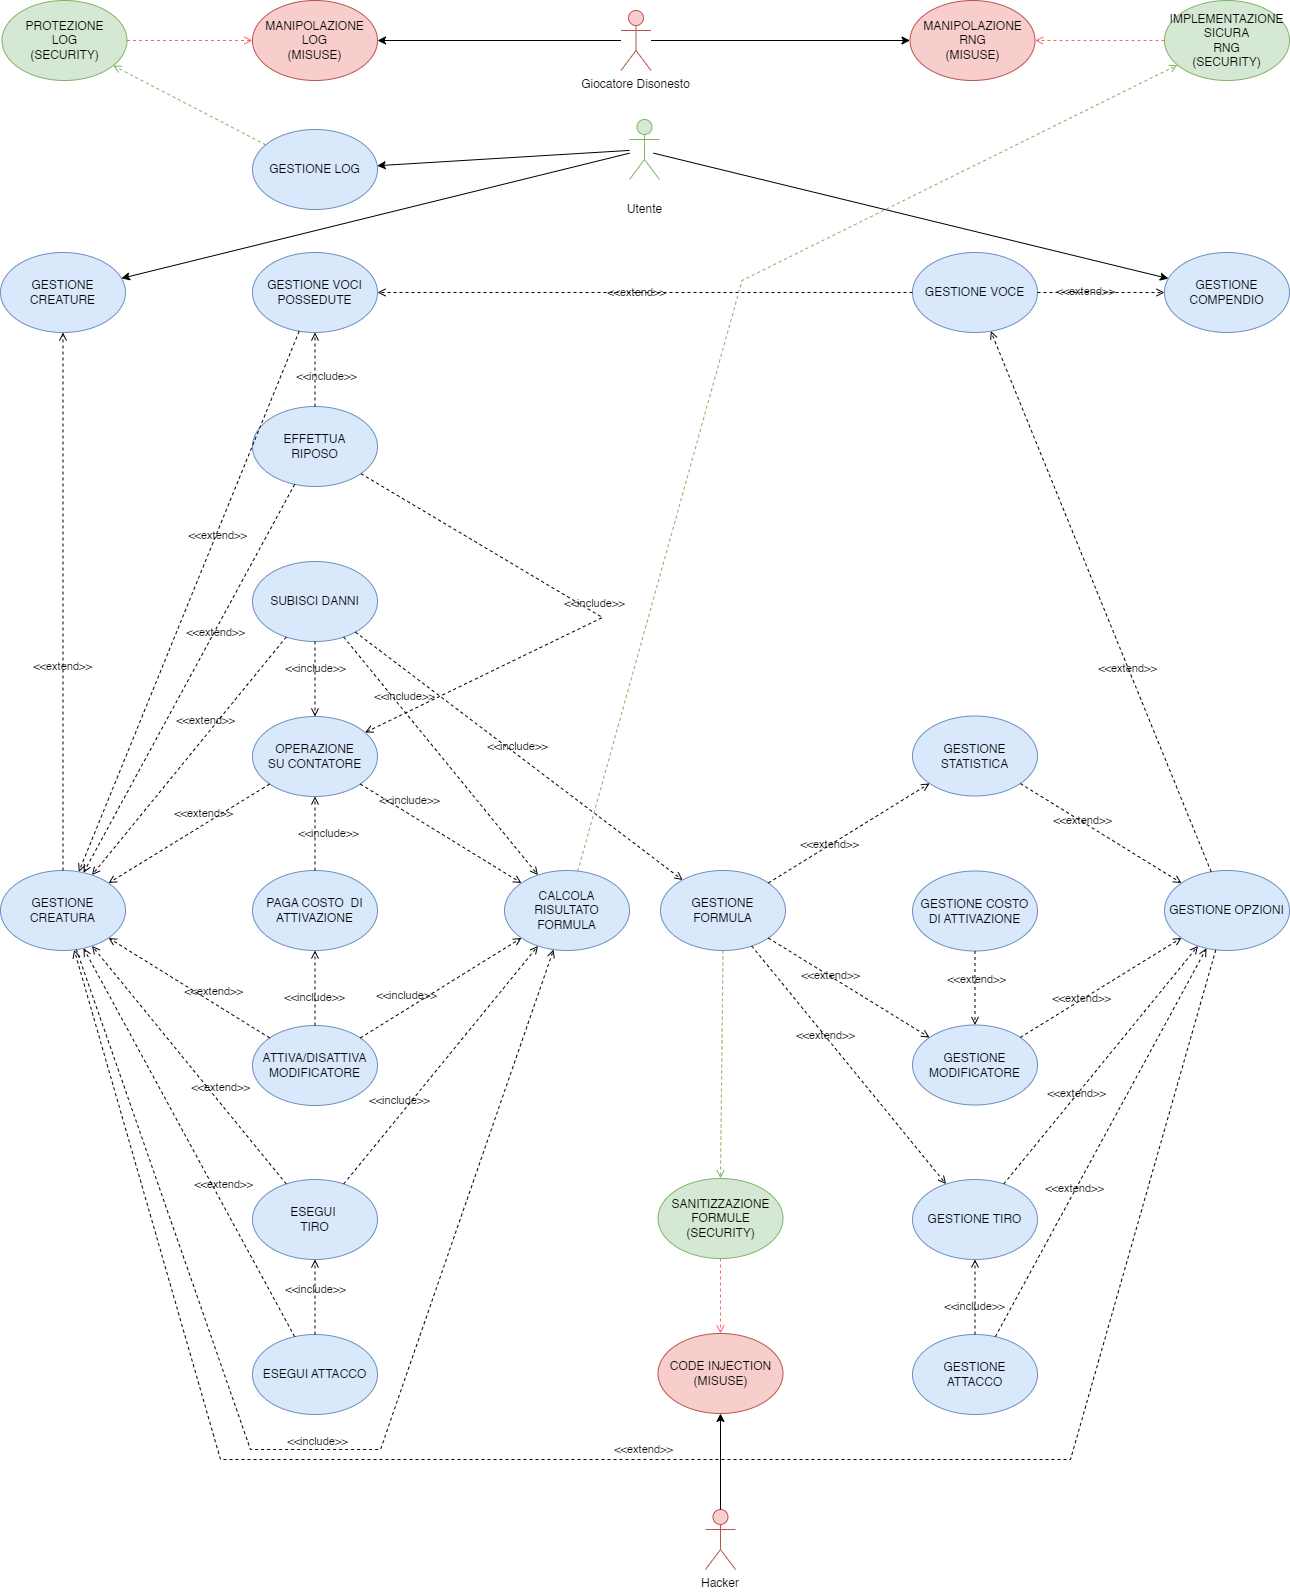
\includegraphics[width=0.9\textwidth,keepaspectratio]{Diagramma CU-Security}
    \label{fig:security}
\end{figure}

\newpage
\begin{table}[h]\small   
\begin{center}
\begin{tabular}{ |p{4cm}|p{11cm}|  }
\hline
\textbf{Titolo} & Protezione Log \\
\hline
\textbf{Descrizione} & I file di log devono essere protetti da manipolazioni per garantire l'integrità e la trasparenza delle operazioni \\
\hline
\textbf{Misuse case} & Manipolazione Log  \\
\hline
\textbf{Relazioni} &  \\
\hline
\textbf{Precondizioni} & L'attaccante ha un accesso parziale o ha scoperto una vulnerabilità nei file di log.  \\
\hline
\textbf{Postcondizioni} & Il sistema protegge i log in modo che ne sia verificabile l'integrità.  \\
\hline
\end{tabular}
    \begin{tabular}{|p{4cm}|p{4.9cm}|p{5cm}|}
        \multirow{3}{=}{\textbf{Scenario principale}} & \textbf{Sistema} & \textbf{Attaccante}\\\cline{2-3}
         & Protegge i file di log in modo che ne sia verificabile l'integrità. &  \\\cline{2-3}
         & & Tenta di modificare o cancellare i file di log per nascondere le sue azioni. \\\cline{2-3}
         & La non integrità dei log è visibile agli altri giocatori, che individuano il tentativo di manipolazione. & \\
         \hline
         \multirow{5}{=}{\textbf{Scenario di attacco avvenuto con successo}} & \textbf{Sistema} & \textbf{Attaccante}\\\cline{2-3}
         & Protegge i file di log in modo che ne sia verificabile l'integrità. &  \\\cline{2-3}
         && L'attaccante riesce a cancellare o alterare i log, nascondendo le tracce delle operazioni disoneste, e riesce a farli apparire integri. \\\cline{2-3}
         & Gli altri giocatori non rilevano la manipolazione dei log. & \\\cline{2-3}
         && Trae vantaggio dalle modifiche disoneste apportate a insaputa degli altri. \\
    \hline
    \end{tabular}
    \end{center}
\end{table}


\clearpage
\begin{table}[h]\small
\begin{center}
\begin{tabular}{ |p{4cm}|p{11cm}|  }
\hline
\textbf{Titolo} & Sanitizzazione Formule \\
\hline
\textbf{Descrizione} & Le formule definite dagli utenti devono essere sanitizzate per prevenire code injection. \\
\hline
\textbf{Misuse case} & Code Injection \\
\hline
\textbf{Relazioni} &  \\
\hline
\textbf{Precondizioni} & L’Attaccante ha i mezzi per eseguire codice malevolo attraverso la possibilità di inserire formule personalizzate fornita dall'applicazione, e le condivide ad altri utenti che le importeranno nella loro applicazione. \\
\hline
\textbf{Postcondizioni} & Il Sistema rileva e blocca l'esecuzione delle formule ritenute potenzialmente dannose. \\
\hline
\end{tabular}
    \begin{tabular}{|p{4cm}|p{4.9cm}|p{5cm}|}
        \multirow{3}{=}{\textbf{Scenario principale}} & \textbf{Sistema} & \textbf{Attaccante}\\\cline{2-3}
        && Condivide con altri utenti formule contenenti codice malevolo, e loro le importano.\\\cline{2-3}
        & Individua il tentativo e sanitizza le formule potenzialmente dannose. & \\\cline{2-3}
         \hline
         \multirow{5}{=}{\textbf{Scenario di attacco avvenuto con successo}} & \textbf{Sistema} & \textbf{Attaccante}\\\cline{2-3}
         && Condivide con altri utenti formule contenenti codice malevolo, e loro le importano.\\\cline{2-3}
         & Non rileva la formula come potenzialmente dannosa e procede nell'esecuzione. & \\\cline{2-3}
         & La formula viene eseguita e potrebbe danneggiare il Sistema. & \\\cline{2-3}
    \hline
    \end{tabular}
\end{center}
\end{table}

\clearpage
\newpage
\subsubsection*{Requisiti di Protezione dei Dati}
Dall’analisi del rischio si possono evincere i seguenti ulteriori requisiti:
\begin{enumerate}[\indent1.]
    \item Creazione di un log per tenere traccia di tutte le azioni svolte dall’Utente sulle creature.
    \item Implementazione di un sistema di sanitizzazione dell’input delle formule personalizzate per impedire l’esecuzione di codice malevolo.
    \item Individuazione di un adeguato sistema di protezione dell’integrità dei log.
\end{enumerate}

\subsubsection{Requisiti di Sistema Aggiornati}

\begin{center}
    \begin{tabular}{ |p{2cm}|p{8cm}|p{3cm}|  }
        \hline
        ID & REQUISITO & TIPO \\ 
        \hline
        R\rf F & Il sistema, tramite un meccanismo di log, tiene traccia di tutte le operazioni eseguite sulle creature & Funzionale \\
        \hline
        R\rf F & Il sistema deve possedere un sistema di sanitizzazione dell'input per le formule personalizzate inserite dall'utente & Funzionale \\\hline
        R\rnf NF & I log devono essere salvaguardati in modo da garantirne l'integrità & Non Funzionale \\
        \hline
    \end{tabular}
\end{center}



\subsubsection{Glossario Aggiornato}

\begin{center}
    \begin{tabular}{ |p{3cm}|p{7cm}|p{3cm}|  }
        \hline
        VOCE & DEFINIZIONE & SINONIMI \\
        \hline
        Log & Registro dove vengono salvate informazioni per tracciare le operazioni eseguite. & Registro \\
        \hline
        Voce di Log & Una singola riga di Log che rappresenta una singola azione effettuata dall'Utente & Riga di Log, Record di Log \\\hline
    \end{tabular}
\end{center}
\vspace{1.5em}
Per soddisfare i nuovi requisiti di sicurezza è stato aggiunto un nuovo caso d’uso “Visualizzazione Log”.

\subsubsection{Scenari Aggiornati}

\begin{center}
    \begin{tabular}{ |p{5cm}|p{9.5cm}|  }
        \hline
        \textbf{Titolo} & Visualizzazione Log \\
        \hline
        \textbf{Descrizione} & L'Utente visualizza i log \\
        \hline
        \textbf{Attori} & Utente \\
        \hline
        \textbf{Relazioni} & \\
        \hline
        \textbf{Precondizioni} &  \\
        \hline
        \textbf{Postcondizioni} & \\
        \hline
        \textbf{Scenario principale} & 
        \begin{enumerate}
            \item L'Utente accede alla sezione di visualizzazione log
            \item Il sistema mostra l'elenco delle azioni effettuate sulle creature
        \end{enumerate}
        \\
        \hline
        \textbf{Scenari alternativi} & \\
        \hline
        \textbf{Requisiti non funzionali} & R23NF\\
        \hline
        \textbf{Punti aperti} &  \\
        \hline
    \end{tabular}
\end{center}



\newpage
\section{Analisi del Problema}
\subsection{Analisi delle Funzionalità}
\subsubsection*{Tabella delle funzionalità}
\begin{center}
    \begin{tabular}{|p{3.5cm}|p{3cm}|p{3cm}|p{3.5cm}|}
        \hline
        \textbf{Funzionalità} & \textbf{Tipo} & \textbf{Grado \newline Complessità} & \textbf{Requisiti \newline Collegati} \\
        \hline
        Gestione \newline Compendio & Gestione Dati, Memorizzazione Dati, Interazione con l’esterno & Complessa & R1F, R2F, R3NF, R4NF, R8NF\\
        \hline
        Gestione Voce & Gestione Dati, Memorizzazione Dati & Complessa & R1F, R9F\\
        \hline
        Gestione Creature & Gestione Dati, Memorizzazione Dati, Interazione con l’esterno & Complessa & R3F, R4F, R5NF, R14NF\\
        \hline
        Gestione Creatura & Gestione Dati, Memorizzazione Dati & Complessa & R3F, R5F, R6F, R7F, R9F, R12F, R13F, R14F, R15F, R16F, R17F, R18F, R1NF, R2NF, R3NF, R4NF, R15NF, R17NF, R18NF\\
        \hline
        Gestione Modificatore & Gestione Dati, Memorizzazione Dati & Complessa & R9F, R10F, R13F, R7NF, R16NF\\
        \hline
        Gestione Statistica & Gestione Dati, Memorizzazione Dati & Complessa & R9F, R10F, R6NF, R16NF\\
        \hline
        Gestione Formula & Gestione Dati, Memorizzazione Dati & Semplice & R8F, R10F, R9NF, R10NF, R11NF, R12NF, R20F\\\hline
        Calcola Risultato Formula & Gestione Dati & Semplice & R11F, R12NF\\\hline
        Visualizzazione Log & Gestione Dati, Interazione con l'esterno & Semplice & R19F, R23NF\\\hline
    \end{tabular}
\end{center}

\vspace{2em}

\setlength{\tabcolsep}{10pt}
\subsubsection*{Gestione Compendio: Tabella Informazioni/Flusso}
\begin{adjustwidth}{-1.5cm}{-1.5cm}
\begin{center}
    \begin{tabular}{|p{3cm}|p{1.5cm}|p{3.5cm}|p{2.5cm}|p{4cm}|}
        \hline
        \textbf{Informazione} & \textbf{Tipo} & \textbf{Livello \newline Protezione/Privacy} & \textbf{Input/Output}&\textbf{Vincoli}\\
        \hline
        Nome Voce & Semplice & Protezione bassa & Output & Massimo 64 caratteri\\\hline
        
    \end{tabular}
\end{center}
\end{adjustwidth}

\vspace{2em}

\subsubsection*{Gestione Voce: Tabella Informazioni/Flusso}
\setlength\LTleft{-1cm}
\setlength\LTright{-1cm}
\begin{center}
    \begin{longtable}{|p{4cm}|p{1.5cm}|p{3.5cm}|p{2.5cm}|p{4cm}|}
        \hline
        \textbf{Informazione} & \textbf{Tipo} & \textbf{Livello \newline Protezione/Privacy} & \textbf{Input/Output}&\textbf{Vincoli}\\
        \hline
        Id & Semplice & Protezione bassa & Output & Massimo 64 caratteri \\
        \hline
        Nome & Semplice & Protezione bassa & Input/Output & Massimo 64 caratteri \\
        \hline
        Descrizione & Semplice & Protezione bassa & Input/Output &  \\
        \hline
        Nome manuale & Semplice & Protezione bassa & Input/Output & Massimo 64 caratteri \\
        \hline        
        Statistiche definite\newline \newline Composte da: 
        \begin{itemize}
            \item Tutte le informazioni incluse in \newline \textbf{Gestione Statistica: Tabella Informazioni/Flusso}
        \end{itemize}& Composto & Protezione bassa & Input/Output &  \\
        \hline
        Statistiche necessarie\newline \newline Composte da: 
        \begin{itemize}
            \item Tutte le informazioni incluse in \newline \textbf{Gestione Statistica: Tabella Informazioni/Flusso}
        \end{itemize}& Composto & Protezione bassa & Input/Output &  \\
        \hline
        Modificatori  \newline \newline Composti da: 
        \begin{itemize}
            \item Tutte le informazioni incluse in \newline \textbf{Gestione Modificatore: Tabella Informazioni/Flusso}
        \end{itemize}& Composto & Protezione bassa & Input/Output &  \\
        \hline
        Numero privilegi \newline selezionabili & Semplice & Protezione bassa & Input/Output & Intero \\
        \hline
        Privilegi selezionabili \newline \newline Composti da:
            \begin{itemize}
                \item Id
                \item Nome
                \item Descrizione
                \item Nome manuale
                \item Statistiche
                \item Modificatori
                \item Numero privilegi \newline selezionabili 
                \item Privilegi \newline selezionabili 
            \end{itemize}
         & Composto & Protezione bassa & Input/Output & Il nome, l'id e il nome manuale possono essere di massimo 64 caratteri\\
        \hline
    \end{longtable}
\end{center}

\vspace{2em}

\subsubsection*{Gestione Creature: Tabella Informazioni/Flusso}
\begin{adjustwidth}{-1.5cm}{-1.5cm}
\begin{center}
    \begin{tabular}{|p{3cm}|p{1.5cm}|p{3.5cm}|p{2.5cm}|p{4cm}|}
        \hline
        \textbf{Informazione} & \textbf{Tipo} & \textbf{Livello \newline Protezione/Privacy} & \textbf{Input/Output}&\textbf{Vincoli}\\
        \hline
        Nome creatura & Semplice & Protezione bassa & Output & Massimo 64 caratteri \\\hline
    \end{tabular}
\end{center}
\end{adjustwidth}

\vspace{2em}

\subsubsection*{Gestione Creatura: Tabella Informazioni/Flusso}
\begin{center}
\setlength\LTleft{-1cm}
\setlength\LTright{-1cm}
    \begin{longtable}{|p{4cm}|p{1.5cm}|p{3cm}|p{2.5cm}|p{4cm}|}
        \hline
        \textbf{Informazione} & \textbf{Tipo} & \textbf{Livello \newline Protezione/\newline Privacy} & \textbf{Input/Output} & \textbf{Vincoli} \\
        \hline
        Id & Semplice & Protezione bassa & Output & Massimo 64 caratteri \\
        \hline
        Nome & Semplice & Protezione bassa & Input/Output & Massimo 64 caratteri \\
        \hline
        Allineamento & Semplice & Protezione bassa & Input/Output & Uno dei valori consentiti come da specifica del vocabolario \\
        \hline
        Voci Possedute \newline \newline Composte da:
        \begin{itemize}
            \item Tutte le informazioni incluse in \textbf{Gestione Voce: Tabella Informazioni/Flusso}
            \item Livello in classe (se è una classe)
            \item Quantità posseduta (se è un oggetto)
        \end{itemize}
        & Composto & Protezione bassa & Input/Output & Id, nome e nome manuale possono essere al massimo di 64 caratteri, il numero privilegi selezionabili, livello in classe e quantità posseduta devono essere interi \\
        \hline
        Statistiche \newline \newline Composte da: \begin{itemize}
            \item Identificatore (Nome o Tipo di Tiro)
            \item Valore
        \end{itemize}& Composto & Protezione bassa & Input/Output & \\
        \hline
        Modificatori posseduti \newline \newline Composti da: 
        \begin{itemize}
            \item Nome
            \item Identificatore associato 
            \item Modifica a formula
        \end{itemize} & Composto & Protezione bassa & Input/Output & \\
        \hline
    \end{longtable}
\end{center}


\vspace{2em}

\subsubsection*{Gestione Modificatore: Tabella Informazioni/Flusso}
\begin{adjustwidth}{-1.5cm}{-1.5cm}
\begin{center}
    \begin{tabular}{|p{3cm}|p{1.5cm}|p{3.5cm}|p{2.5cm}|p{4cm}|}
        \hline
        \textbf{Informazione} & \textbf{Tipo} & \textbf{Livello \newline Protezione/Privacy} & \textbf{Input/Output}&\textbf{Vincoli}\\
        \hline
        Nome & Semplice & Protezione bassa & Input/Output & Massimo 64 caratteri \\\hline
        Identificatore associato & Semplice & Protezione bassa & Input/Output & \\\hline
        Modifica a \newline Formula & Semplice & Protezione bassa & Input/Output & Stringa \\\hline
    \end{tabular}
\end{center}
\end{adjustwidth}
        
\vspace{2em}

\newpage

\subsubsection*{Gestione Statistica: Tabella Informazioni/Flusso}
\begin{center}
\setlength\LTleft{-0.5cm}
\setlength\LTright{-1cm}
    \begin{longtable}{|p{3cm}|p{1.5cm}|p{3.5cm}|p{2.5cm}|p{4cm}|}
        \hline
        \textbf{Informazione} & \textbf{Tipo} & \textbf{Livello \newline Protezione/Privacy} & \textbf{Input/Output}&\textbf{Vincoli}\\
        \hline
        Nome & Semplice & Protezione bassa & Input/Output & Ogni nome deve poter essere usato per identificare una Statistica in modo univoco \\\hline
        Tipo di Tiro \newline \newline Composto da: 
        \begin{itemize}
            \item Oggetto usato
            \item Caratteristica usata
            \item Sottotipo
            \item Attributi del sottotipo
        \end{itemize}& Composto & Protezione bassa & Input/Output & Ogni Tipo di Tiro deve poter essere usato per identificare una Statistica in modo univoco\\\hline
        Valore & Composto & Protezione bassa & Input/Output & Rappresentato tramite una formula o una serie di formule, ciascuna associata a un numero intero e a una specifica Statistica senza Tiri di dado. In questo caso, il valore della Statistica viene determinato dalla formula corrispondente all'intero, che rappresenta il valore della Statistica di riferimento. \\\hline
        Formula \newline \newline Composta da: 
        \begin{itemize}
            \item Id
            \item Valore massimo
            \item Valore minimo
            \item Formula in stringa
        \end{itemize}& Composto & Protezione bassa & Output & Formula valida come da specifiche dei requisiti e del vocabolario, id di massimo 64 caratteri \\\hline
    \end{longtable}
\end{center}

\vspace{2em}

\subsubsection*{Gestione Formula: Tabella Informazioni/Flusso}
\begin{adjustwidth}{-1.5cm}{-1.5cm}
\begin{center}
    \begin{tabular}{|p{3cm}|p{1.5cm}|p{3.5cm}|p{2.5cm}|p{4cm}|}
        \hline
        \textbf{Informazione} & \textbf{Tipo} & \textbf{Livello \newline Protezione/Privacy} & \textbf{Input/Output}&\textbf{Vincoli}\\
        \hline
         Id Formula& Semplice & Protezione bassa & Output & Massimo 64 caratteri \\\hline
        Valore minimo & Semplice & Protezione bassa & Input/Output & Intero \\\hline
        Valore massimo & Semplice & Protezione bassa & Input/Output & Intero \\\hline
        Formula in stringa & Semplice & Protezione bassa & Input/Output & Stringa valida come da specifiche dei requisiti e del vocabolario \\\hline
    \end{tabular}
\end{center}
\end{adjustwidth}

\vspace{2em}

\subsubsection*{Calcola Risultato Formula: Tabella Informazioni/Flusso}
\begin{adjustwidth}{-1.5cm}{-1.5cm}
\begin{center}
    \begin{tabular}{|p{3cm}|p{1.5cm}|p{3.5cm}|p{2.5cm}|p{4cm}|}
        \hline
        \textbf{Informazione} & \textbf{Tipo} & \textbf{Livello \newline Protezione/Privacy} & \textbf{Input/Output}&\textbf{Vincoli}\\
        \hline
        Formula \newline \newline Composta da: 
        \begin{itemize}
            \item Id
            \item Valore massimo
            \item Valore minimo
            \item Formula in stringa
        \end{itemize}& Composto & Protezione bassa & Output & Formula valida come da specifiche dei requisiti e del vocabolario, id di massimo 64 caratteri \\\hline
        Modificatori applicabili \newline \newline Composti da: 
        \begin{itemize}
            \item Nome
            \item Identificatore associato 
            \item Modifica a formula
        \end{itemize} & Composto & Protezione bassa & Input/Output & \\
        \hline
    \end{tabular}
\end{center}
\end{adjustwidth}

\vspace{2em}

\subsubsection*{Visualizzazione Log: Tabella Informazioni/Flusso}
\begin{adjustwidth}{-1.5cm}{-1.5cm}
\begin{center}
    \begin{tabular}{|p{3cm}|p{1.5cm}|p{3.5cm}|p{2.5cm}|p{4cm}|}
        \hline
        \textbf{Informazione} & \textbf{Tipo} & \textbf{Livello \newline Protezione/Privacy} & \textbf{Input/Output}&\textbf{Vincoli}\\
        \hline
        Voce di Log \newline Composta da: \begin{itemize}
            \item Timestamp
            \item Nuovo stato della creatura
        \end{itemize} & Composto & Protezione alta & Output & \\\hline
    \end{tabular}
\end{center}
\end{adjustwidth}

\clearpage
\newpage
\subsection{Analisi dei Vincoli}
\subsubsection*{Tabella vincoli}
\begin{center}
    \begin{tabular}{|p{3cm}|p{3cm}|p{3.5cm}|p{4cm\RaggedRight}|}
        \hline
        \textbf{Requisito} & \textbf{Categoria} & \textbf{Impatto} & \textbf{Funzionalità} \\
        \hline
        Velocità di \newline memorizzazione dei dati & Tempo di risposta & Cercare di migliorare & Gestione Compendio, Gestione Voce, \newline Gestione Creature, Gestione Creatura, Gestione Statistica, Gestione Modificatore \\
        \hline
        Semplicità di navigazione nell'applicazione & Usabilità & Cercare di migliorare & Gestione Compendio, Gestione Voce, \newline Gestione Creature, Gestione Creatura, Gestione Statistica, Gestione Modificatore, \newline Visualizzazione Log \\
        \hline
        Ottimizzazione del tempo di aggiornamento delle interfacce al cambiamento di stato & Tempo di risposta & Cercare di migliorare & Gestione Compendio, Gestione Voce, \newline Gestione Creature, Gestione Creatura, Gestione Statistica, Gestione Modificatore, Calcola Risultato Formula \\
        \hline
        Facile \newline manutenibilità ed estensione futura & Riusabilità & Peggioramento tempo di risposta, aumento del numero di entità & Gestione Compendio, Gestione Voce, \newline Gestione Creature, Gestione Creatura, Gestione Statistica, Gestione Modificatore, Calcola Risultato Formula \\
        \hline
    \end{tabular}
\end{center}

\clearpage
\newpage
\subsection{Analisi delle Interazioni}
\subsubsection*{Tabella maschere}
\begin{adjustwidth}{-1.5cm}{-1.5cm}
    \begin{center}
        \begin{longtable}{|p{5cm}|p{5cm}|p{5cm}|}
        \hline
        \textbf{Maschera} & \textbf{Informazioni} & \textbf{Funzionalità} \\ \hline
        Home Compendio & 
        \textbf{Navigazione verso:} 
        \begin{itemize}
            \item View Crea Voce 
            \item View Elimina Voce 
            \item View Importa/Esporta Voci
        \end{itemize}
        \textbf{Visualizzazione di (per ogni voce):}
        \begin{itemize}
            \item View Voce
        \end{itemize} & 
        Gestione Compendio \\ \hline
        
        View Crea Voce & 
        \textbf{Visualizzazione di:}
        \begin{itemize}
            \item Finestra di dialogo con richiesta di conferma
            \item View Voce
        \end{itemize} & 
        Gestione Compendio \\ \hline
        
        View Elimina Voce & 
        \textbf{Visualizzazione di:}
        \begin{itemize}
            \item Nome voce
            \item Nome manuale
            \item Finestra di dialogo con richiesta di conferma
        \end{itemize} & 
        Gestione Compendio \\ \hline
        
        View Importa/Esporta Voci & 
        \textbf{Navigazione verso:}
        \begin{itemize}
            \item Esplora risorse del sistema sottostante
        \end{itemize}
        \textbf{Visualizzazione di:}
        \begin{itemize}
            \item Tipo di operazione che si sta svolgendo
            \item Finestra di dialogo con richiesta di conferma per scelta file
        \end{itemize} & 
        Gestione Compendio \\ \hline
        
        View Voce & 
        \textbf{Navigazione verso:}
        \begin{itemize}
            \item View Crea Voce
            \item View Elimina Voce
        \end{itemize}
        \textbf{Visualizzazione di (per ogni privilegio selezionabile):}
        \begin{itemize}
            \item View Voce
        \end{itemize}
        \textbf{Visualizzazione di (per ogni statistica):}
        \begin{itemize}
            \item View Statistica
        \end{itemize}
        \textbf{Visualizzazione di (per ogni modificatore):}
        \begin{itemize}
            \item View Modificatore
        \end{itemize}
        \textbf{Visualizzazione (con possibilità di modifica) di:}
        \begin{itemize}
            \item Nome Manuale
            \item Nome
            \item Descrizione
            \item Innesco scelta Privilegi
            \item Numero Privilegi Selezionabili
        \end{itemize}
        \textbf{Visualizzazione (con possibilità di modifica) di (se oggetto):}
        \begin{itemize}
            \item Tipo oggetto
        \end{itemize} & 
        Gestione Voce \\ \hline
        
        View Crea Statistica & 
        \textbf{Visualizzazione di:}
        \begin{itemize}
            \item Finestra di dialogo con richiesta di conferma
        \end{itemize} &  Gestione Voce
        \\ \hline
        
        View Elimina Statistica & 
        \textbf{Visualizzazione di:}
        \begin{itemize}
            \item Finestra di dialogo con richiesta di conferma
            \item Nome o tipo di tiro per identificare la statistica
        \end{itemize} & Gestione Voce
        \\ \hline

        View Crea Modificatore & 
        \textbf{Visualizzazione di:}
        \begin{itemize}
            \item Finestra di dialogo con richiesta di conferma
        \end{itemize} & Gestione Voce
        \\ \hline

        View Elimina Modificatore & 
        \textbf{Visualizzazione di:}
        \begin{itemize}
            \item Finestra di dialogo con richiesta di conferma
            \item Nome modificatore
        \end{itemize} & Gestione Voce
        \\ \hline
        
        View Formula & 
        \textbf{Visualizzazione (con possibilità di modifica) di:}
        \begin{itemize}
            \item Formula in stringa
            \item Minimo
            \item Massimo
        \end{itemize} & 
         Gestione Formula \\\hline
        
        View Statistica & \textbf{Navigazione verso:}
        \begin{itemize}
            \item View Crea Formula
            \item View Elimina Formula 
            \item View Crea Mappa di Valori
            \item View Elimina Mappa di Valori
        \end{itemize}
        \textbf{Visualizzazione (con possibilità di modifica) di:}
        \begin{itemize}
            \item Attributi del Tipo
        \end{itemize}
        \textbf{Visualizzazione di (se statistica con mappa di valori):}
        \begin{itemize}
            \item View Mappa di Valori
        \end{itemize}
        \textbf{Visualizzazione di (se statistica semplice):}
        \begin{itemize}
            \item View Formula
        \end{itemize} & Gestione Statistica
        \\ \hline
        
        View Mappa di Valori & 
        \textbf{Visualizzazione (con possibilità di modifica) di:}
        \begin{itemize}
            \item Nome statistica referenziata
        \end{itemize}
        \textbf{Visualizzazione (con possibilità di modifica) di (per ogni entry):}
        \begin{itemize}
           \item Valore Statistica referenziata
            \item View Formula (corrispondente)
        \end{itemize} & Gestione Formula
        \\ \hline

        View Crea Formula  & 
        \textbf{Visualizzazione di:}
        \begin{itemize}
            \item Finestra di dialogo con richiesta di conferma
        \end{itemize} & Gestione Statistica
        \\ \hline

        View Elimina Formula  & 
        \textbf{Visualizzazione di:}
        \begin{itemize}
            \item Finestra di dialogo con richiesta di conferma
            \item Id formula
        \end{itemize} & Gestione Statistica
        \\ \hline 

        View Crea Mappa di Valori & 
        \textbf{Visualizzazione di:}
        \begin{itemize}
            \item Finestra di dialogo con richiesta di conferma
        \end{itemize} & Gestione Statistica
        \\ \hline

        View Elimina Mappa di Valori & 
        \textbf{Visualizzazione di:}
        \begin{itemize}
            \item Finestra di dialogo con richiesta di conferma
            \item Id Formula
        \end{itemize} & Gestione Statistica
        \\ \hline
        
        View Modificatore & 
        \textbf{Visualizzazione di:}
        \begin{itemize}
            \item Parola chiave per vecchia formula
            \item Attributi statistiche a cui si applica
        \end{itemize}
        \textbf{Visualizzazione di (se modificatore non cumulabile):}
        \begin{itemize}
            \item Tipo di modificatore non cumulabile
        \end{itemize}
        \textbf{Visualizzazione di (se modificatore cumulabile):}
        \begin{itemize}
            \item Stringa che rappresenta modifica
        \end{itemize} &  Gestione Modificatore\\ \hline

        
        Home Creature & \textbf{Navigazione verso:}
        \begin{itemize}
            \item View Crea Creatura
            \item View Elimina Creatura
            \item View Duplica Creatura
            \item View Importa/Esporta Creatura
            \item Home Gestione Creatura
        \end{itemize}
        \textbf{Visualizzazione di (per ogni creatura):}
        \begin{itemize}
            \item Nome 
            \item Voci principali della creatura (Razza, Classi e Livello per ogni classe)
        \end{itemize} & Gestione Creature \\ \hline
        
        View Crea Creatura & \textbf{Visualizzazione di:}
        \begin{itemize}
            \item Campo nome creatura da riempire
            \item Finestra di dialogo con richiesta di conferma
        \end{itemize} & Gestione Creature \\ \hline
        
        View Elimina Creatura & \textbf{Visualizzazione di:}
        \begin{itemize}
            \item Finestra di dialogo con richiesta di conferma
            \item Id creatura
        \end{itemize} & Gestione Creature \\ \hline
        
        View Duplica Creatura & \textbf{Visualizzazione di:}
        \begin{itemize}
            \item Finestra di dialogo con richiesta di conferma
            \item Id creatura
        \end{itemize} & Gestione Creature \\ \hline
        
        View Importa/ Esporta Creatura & \textbf{Navigazione verso:}
        \begin{itemize}
            \item Esplora risorse del sistema sottostante
        \end{itemize}
        \textbf{Visualizzazione di:}
        \begin{itemize}
            \item Tipo di operazione che si sta svolgendo
            \item Finestra di dialogo con richiesta di conferma per scelta file
        \end{itemize} & Gestione Creature \\ \hline
        
        Home Gestione Creatura & 
        \textbf{Visualizzazione (con possibilità di modifica) di:}
        \begin{itemize}
            \item Nome
            \item Allineamento
        \end{itemize}
        \textbf{Visualizzazione di:}
        \begin{itemize}
            \item View Gestione Voci Possedute
        \end{itemize}
        \textbf{Visualizzazione di (per ogni statistica):}
        \begin{itemize}
            \item View Statistica 
            \item Modificatori applicati
            \item Risultato statistica
        \end{itemize}
        \textbf{Visualizzazione di (per ogni modificatore posseduto):}
        \begin{itemize}
            \item View Modificatore (posseduto)
            \item Se attivo o no
        \end{itemize}
        \textbf{Navigazione verso:} 
        \begin{itemize}
            \item View Subisci Danni
            \item View Effettua Riposo
            \item View Attiva/Disattiva Modificatore
        \end{itemize} & Gestione Creatura \\ \hline
        
        View Gestione Voci Possedute & \textbf{Navigazione verso:}
        \begin{itemize}
            \item View Prendi Voce
            \item View Rimuovi Voce
        \end{itemize}
        \textbf{Visualizzazione di (per ogni voce posseduta):}
        \begin{itemize}
            \item View Voce Posseduta
        \end{itemize} & Gestione Creatura \\ \hline
        
        View Prendi Voce & \textbf{Visualizzazione di (per ogni voce del compendio):}
        \begin{itemize}
            \item View Voce
            \item Casella di selezione
        \end{itemize}
        \textbf{Visualizzazione di (per ogni voce eventualmente sostituita):}
        \begin{itemize}
            \item View Voce
        \end{itemize} & Gestione Creatura \\ \hline
        
        View Rimuovi Voce & \textbf{Visualizzazione di:}
        \begin{itemize}
            \item Finestra di dialogo per conferma
            \item Id voce
        \end{itemize} & Gestione Creatura \\ \hline
        
        View Voce Posseduta & 
        \textbf{Visualizzazione di:}
        \begin{itemize}
            \item View Voce
        \end{itemize}
        \textbf{Navigazione verso:}
        \begin{itemize}
            \item View Seleziona Privilegi
        \end{itemize}
        \textbf{Visualizzazione (con possibilità di modifica) di:}
        \begin{itemize}
            \item Nome
            \item Attributo Voce Posseduta (livello o quantità)
        \end{itemize}
        \textbf{Visualizzazione di (per ogni privilegio selezionato):}
        \begin{itemize}
            \item View Voce Posseduta
        \end{itemize} & Gestione Creatura \\ \hline
        
        View Seleziona Privilegi & \textbf{Visualizzazione di:}
        \begin{itemize}
            \item Numero privilegi selezionabili
            \item Numero Privilegi selezionati
            \item Finestra di dialogo per conferma
        \end{itemize}
        \textbf{Visualizzazione di (per ogni privilegio selezionabile):}
        \begin{itemize}
            \item View Voce
            \item Casella di selezione
        \end{itemize} & Gestione Creatura \\ \hline
        
        View Subisci Danni & \textbf{Navigazione verso:}
        \begin{itemize}
            \item View Calcola Risultato
        \end{itemize}
        \textbf{Visualizzazione (con possibilità di modifica) di:}
        \begin{itemize}
            \item View Formula
            \item Tipo di Danno
            \item È danno magico
        \end{itemize} & Gestione Creatura \\ \hline
        
        View Attiva/Disattiva Modificatore & \textbf{Visualizzazione di:}
        \begin{itemize}
            \item View Modificatore
        \end{itemize}
        \textbf{Visualizzazione (con possibilità di modifica) di:}
        \begin{itemize}
            \item Stato attivazione
        \end{itemize} & Gestione Creatura \\ \hline

        View Effettua Riposo & 
        \textbf{Richiesta di:}
        \begin{itemize}
            \item Tipo Riposo
        \end{itemize} 
        
        \textbf{Visualizzazione di:}
        \begin{itemize}
            \item Finestra di dialogo per conferma
        \end{itemize} 
        
        \textbf{Visualizzazione di (per ogni voce che dichiara il riposo selezionato):}
        \begin{itemize}
            \item View Selezione Privilegi
        \end{itemize} & Gestione Creatura \\ \hline
        
        View Risultato Formula &
        \textbf{Visualizzazione di:}
        \begin{itemize}
            \item View Formula
            \item Risultato
        \end{itemize}
        \textbf{Visualizzazione di (per ogni modificatore che si applica):}
        \begin{itemize}
            \item View Modificatore 
        \end{itemize} & Calcola Risultato Formula\\ \hline
        
        View Log & 
        \textbf{Visualizzazione di:}
        \begin{itemize}
            \item Log delle modifiche
        \end{itemize} & Visualizzazione Log \\ \hline

        \end{longtable}
    \end{center}
\end{adjustwidth}

\subsubsection*{Tabella Sistemi Esterni}
\begin{adjustwidth}{-1.5cm}{-1.5cm}
\begin{center}
    \begin{tabular}{|p{2.5cm}|p{5cm}|p{4cm}|p{4cm}|}
        \hline
        \textbf{Sistema} & \textbf{Descrizione} & \textbf{Protocollo di \newline Interazione} & \textbf{Livello di Sicurezza} \\ \hline
        Esplora Risorse & Sistema che si occupa della gestione di un filesystem & Rende disponibile un’interfaccia grafica per la visualizzazione e modifica di file in un filesystem & Basso livello di sicurezza essendo accessibile da chiunque \\ \hline
    \end{tabular}
\end{center}
\end{adjustwidth}


\clearpage
\newpage
\subsection{Analisi Ruoli e Responsabilità}
\subsubsection*{Tabella Ruoli}
\begin{adjustwidth}{-1cm}{-1cm}
\begin{center}
    \begin{tabular}{|p{1.5cm}|p{5cm}|p{3cm}|p{2.5cm}|p{2.5cm}|}
        \hline
        \textbf{Ruolo} & \textbf{Responsabilità} & \textbf{Maschere} & \textbf{Riservatezza} & \textbf{Numerosità} \\\hline
        Utente & Gestire le proprie creature in modo coerente con le voci \newline esistenti nel compendio, \newline garantire che le voci del \newline compendio create siano sicure da usare (ovvero non \newline contengano formule malevole) & Tutte le maschere nella \textbf{Tabella maschere} & È richiesto un medio grado di riservatezza & Nessun vincolo \\\hline
    \end{tabular}
\end{center}
\end{adjustwidth}
\subsubsection*{Utente: tabella ruolo-informazioni}
\begin{adjustwidth}{-0.5cm}{-0.5cm}
    \begin{tabular}{|l|l|}
        \hline
        \textbf{Informazione} & \textbf{Tipo di Accesso} \\
        \hline
        Id Voce Compendio& Lettura \\
        \hline
        Nome Voce Compendio& Lettura/Scrittura \\
        \hline
        Descrizione Voce Compendio& Lettura/Scrittura \\
        \hline
        Nome manuale & Lettura/Scrittura \\
        \hline
        Statistiche & Lettura/Scrittura \\
        \hline
        Modificatori & Lettura/Scrittura \\\hline
        Numero privilegi selezionabili & Lettura/Scrittura \\
        \hline
        Privilegi selezionabili & Lettura/Scrittura \\
        \hline
        Id creatura & Lettura \\
        \hline
        Nome creatura & Lettura/Scrittura \\
        \hline
        Allineamento & Lettura/Scrittura \\
        \hline
        Voci possedute & Lettura/Scrittura \\
        \hline
        Nome Statistica & Lettura/Scrittura \\\hline
        Tipo di Tiro associato a Statistica & Lettura/Scrittura \\\hline
        Valore & Lettura/Scrittura \\\hline
        Nome modificatore & Lettura/Scrittura \\\hline
        Identificatore associato a Modificatore & Lettura/Scrittura \\\hline
        Modifica a formula & Lettura/Scrittura \\\hline
        Valore massimo formula & Lettura/Scrittura \\
        \hline
        Valore minimo formula & Lettura/Scrittura \\
        \hline
        Formula & Lettura/Scrittura \\
        \hline
        Voce di Log & Lettura \\
        \hline
    \end{tabular}
\end{adjustwidth}


\clearpage
\newpage
\subsection{Scomposizione del Problema}
\subsubsection*{Tabella Scomposizione Funzionalità}
\begin{adjustwidth}{-1cm}{-1cm}
\begin{center}
    \begin{tabular}{|c|p{11cm}|}
        \hline
        \textbf{Funzionalità} & \textbf{Scomposizione} \\\hline
        Gestione Compendio & Aggiunta Voce, Eliminazione Voce, Importazione Voce, \newline Esportazione Voce, Gestione Voce \\\hline
        Gestione Voce & Visualizzazione Voce, Modifica Voce, Gestione Statistica, Gestione Modificatore, Aggiunta Statistica, Eliminazione Statistica, Aggiunta Modificatore, Eliminazione Modificatore \\\hline
        Gestione Modificatore & Gestione Formula \\\hline
        Gestione Statistica & Gestione Formula \\\hline
        Gestione Creature & Creazione Creatura, Eliminazione Creatura, Duplicazione Creatura, Importazione Creatura, Esportazione Creatura \\\hline
        Gestione Creatura & Gestione Voci Possedute, Effettua Riposo, Subisci Danni, \newline Attiva/Disattiva Modificatore\\\hline
        Gestione Voci Possedute & Prendi Voce, Rimuovi Voce, Seleziona Privilegi \\\hline
    \end{tabular}
\end{center}
\end{adjustwidth}

\vspace{2em}

\subsubsection*{Tabella Sotto-Funzionalità: Gestione Compendio}
\begin{adjustwidth}{-1cm}{-1cm}
\begin{center}
    \begin{tabular}{|p{4cm}|p{4cm}|p{4cm}|p{2.5cm}|}
        \hline
        \textbf{Sotto-Funzionalità} & \textbf{Sotto-Funzionalità} & \textbf{Legame} & \textbf{Informazioni} \\\hline
        Eliminazione Voce & Aggiunta Voce, Importazione Voce & Non si può eliminare una voce che non sia stata creata o importata in precedenza & Id voce \\\hline
        Esportazione Voce & Aggiunta Voce, Importazione Voce & Non si può esportare una voce che non sia stata creata o importata in precedenza & Id voce \\\hline
        Gestione Voce & Aggiunta Voce, Importazione Voce & Non si può gestire una voce che non sia stata creata o importata in precedenza & Id voce \\\hline
    \end{tabular}
\end{center}
\end{adjustwidth}

\vspace{2em}

\subsubsection*{Tabella Sotto-Funzionalità: Gestione Voce}
\begin{adjustwidth}{-1cm}{-1cm}
\begin{center}
    \begin{tabular}{|p{4cm}|p{4cm}|p{4cm}|p{2.5cm}|}
        \hline
        \textbf{Sotto-Funzionalità} & \textbf{Sotto-Funzionalità} & \textbf{Legame} & \textbf{Informazioni} \\\hline
        Gestione Statistica, \newline Eliminazione Statistica & Aggiunta Statistica & Si può gestire o eliminare solo una statistica che sia stata precedentemente aggiunta & Identificatore statistica \\\hline
        Gestione Modificatore, \newline Eliminazione Modificatore & Aggiunta Modificatore & Si può gestire o eliminare solo un modificatore che sia stato precedentemente aggiunto & Nome modificatore \\\hline
    \end{tabular}
\end{center}
\end{adjustwidth}

\vspace{2em}

\subsubsection*{Tabella Sotto-Funzionalità: Gestione Creature}
\begin{adjustwidth}{-1cm}{-1cm}
\begin{center}
    \begin{tabular}{|p{4cm}|p{4cm}|p{4cm}|p{2.5cm}|}
        \hline
        \textbf{Sotto-Funzionalità} & \textbf{Sotto-Funzionalità} & \textbf{Legame} & \textbf{Informazioni} \\\hline
        Eliminazione Creatura & Creazione Creatura, Importazione Creatura & Non si può eliminare una creatura che non sia stata creata o importata in precedenza & Id creatura \\\hline
        Duplicazione Creatura & Creazione Creatura, Importazione Creatura & Non si può duplicare una creatura che non sia stata creata o importata in precedenza & Id creatura \\\hline
        Esportazione Creatura & Creazione Creatura, Importazione Creatura & Non si può esportare una creatura che non sia stata creata o importata in precedenza & Id creatura \\\hline
    \end{tabular}
\end{center}
\end{adjustwidth}

\vspace{2em}

\subsubsection*{Tabella Sotto-Funzionalità: Gestione Voci Possedute}
\begin{adjustwidth}{-1cm}{-1cm}
\begin{center}
    \begin{tabular}{|p{4cm}|p{4cm}|p{4cm}|p{2.5cm}|}
        \hline
        \textbf{Sotto-Funzionalità} & \textbf{Sotto-Funzionalità} & \textbf{Legame} & \textbf{Informazioni} \\\hline
        Rimuovi Voce & Prendi Voce & Si può rimuovere una voce solo se è stata precedentemente presa & Id voce \\\hline
        Seleziona Privilegi & Prendi Voce & Si possono selezionare i privilegi dati da una voce solo se è stata precedentemente presa & Id voce \\\hline
    \end{tabular}
\end{center}
\end{adjustwidth}
\vspace{1em}
\textbf{Nota}: Per alcune funzionalità non è presente alcuna tabella di sotto-funzionalità poiché tra le relative sotto-funzionalità non vi è alcun legame.

\clearpage
\newpage
\subsection{Modello del Dominio}
Di seguito è riportato il diagramma delle classi che rappresenta la parte del modello del dominio relativa alle creature.
\begin{figure}[h!]
    \centering
    \includegraphics[width=0.6\textwidth,keepaspectratio]{DominioCreatura.png}
    \label{fig:dominioCreatura}
\end{figure}
\newline

\clearpage
\newpage
Di seguito è riportato il diagramma delle classi che rappresenta la parte del modello del dominio relativa alle statistiche tramite le quali vengono definite le Formule. 
\begin{figure}[h!]
    \centering
    \includegraphics[width=0.8\textwidth,keepaspectratio]{DominioStatistica.png}
    \label{fig:dominioStat}
\end{figure}
\newline

\clearpage
\newpage
Di seguito è riportato il diagramma delle classi che rappresenta la parte del modello del dominio relativa alle voci del compendio. I tipi di Oggetto sono predefiniti nel gioco.
\begin{figure}[h!]
    \centering
    \includegraphics[width=0.8\textwidth,keepaspectratio]{DominioVoce.png}
    \label{fig:dominioVoce}
\end{figure}
\newline 
Di seguito è riportato il diagramma delle classi che rappresenta la parte del modello del dominio relativa alle formule.
\begin{figure}[h!]
    \centering
    \includegraphics[width=0.6\textwidth,keepaspectratio]{DominioFormula.png}
    \label{fig:dominioFormula}
\end{figure}
\clearpage
\newpage
Di seguito è riportato il diagramma delle classi che rappresenta la parte del modello del dominio relativa ai modificatori e identificatori. I Modificatori modificano la formula associata a un gruppo di statistiche, identificato tramite Identificatore.
\begin{figure}[h!]
\makebox[\textwidth][c]{
    \centering
    \includegraphics[width=1.2\textwidth,keepaspectratio]{DominioMod.png}
    \label{fig:dominioMod}
} 
\end{figure}

\clearpage
\newpage
\subsection{Architettura Logica: Struttura}
\subsubsection{Diagramma dei package}
\vspace{1em}
\begin{figure}[h!]
    \centering
    \includegraphics[width=1\textwidth,keepaspectratio]{ANALISI Diagramma dei Package}
    \label{fig:packageAnalisi}
\end{figure}
\subsubsection*{Diagramma delle classi: Dominio}
Non viene riportato il diagramma delle classi associato al package Dominio in quanto è il modello del dominio creato precedentemente.
\subsubsection*{Diagramma delle classi: Log}
\begin{figure}[h!]
    \centering
    \includegraphics[width=0.8\textwidth,keepaspectratio]{classiLog.png}
    \label{fig:classiLog}
\end{figure}

\clearpage
\newpage
\subsection{Architettura Logica: Interazione}
\subsubsection*{Diagramma di sequenza: SubisciDanni}
\begin{figure}[h!]
    \centering
    \includegraphics[width=1\textwidth,keepaspectratio]{seqSubisciDanni.png}
    \label{fig:subisciDanni}
\end{figure}
\subsubsection*{Diagramma di sequenza: SelezionaPrivilegi}
\begin{figure}[h!]
    \centering
    \includegraphics[width=1\textwidth,keepaspectratio]{seqSelezionaPrivilegi.png}
    \label{fig:selezionaPrivilegi}
\end{figure}

\clearpage
\newpage
\subsubsection*{Diagramma di sequenza: EffettuaRiposo}
\begin{figure}[h!]
    \centering
    \includegraphics[width=1\textwidth,keepaspectratio]{seqEffettuaRiposo.png}
    \label{fig:effettuaRiposo}
\end{figure}

\clearpage
\newpage
\subsubsection*{Diagramma di sequenza: CalcolaRisultato}
\begin{figure}[h!]
    \centering
    \includegraphics[width=1\textwidth,keepaspectratio]{seqCalcolaRisultato.png}
    \label{fig:calcolaRisultato}
\end{figure}
\newpage
\clearpage
\subsubsection*{Diagramma di sequenza: MostraStatistiche}
\begin{figure}[h!]
    \centering
    \includegraphics[width=0.6\textwidth,keepaspectratio]{seqMostraStatistiche.png}
    \label{fig:mostraStatistiche}
\end{figure}
\subsection{Architettura Logica: Comportamento}
Dopo un’analisi del sistema, riteniamo che non esistano entità nel progetto che richiedano un diagramma di stato.

\clearpage
\newpage
\subsection{Piano di Lavoro}
Il progetto e lo sviluppo del sistema sono assegnati a diversi team come indicato nella tabella sottostante:
\begin{center}
    \begin{tabular}{|c|c|}
        \hline
        \textbf{Nome Team} & \textbf{Composizione} \\\hline
        Team Progettazione & Bacchelli, Bufalini \\\hline
        Team Sviluppo A & Bacchelli \\\hline
        Team Sviluppo B & Bufalini \\\hline
        Team DB & Bacchelli, Bufalini \\\hline
        Team Sicurezza & Bacchelli, Bufalini \\\hline
        Team Grafico & Bacchelli, Bufalini \\
        \hline 
    \end{tabular}
\end{center}

\vspace{2em}

\begin{adjustwidth}{-1.5cm}{-1.5cm}
    \begin{center}
    \begin{longtable}{|p{6cm}|p{4.5cm}|p{4.5cm}|}
        \hline
        \textbf{Package} & \textbf{Progetto} & \textbf{Sviluppo} \\\hline
        Dominio & Team Progettazione + Team DB & Team Sviluppo A + Team Sviluppo B + Team DB\\\hline
        GestioneCompendio & Team Progettazione & Team Sviluppo A\\\hline
        GestioneVoce & Team Progettazione & Team Sviluppo A\\\hline
        GestioneCreature & Team Progettazione & Team Sviluppo B\\\hline
        GestioneCreatura& Team Progettazione & Team Sviluppo B\\\hline
        GestioneModificatore & Team Progettazione & Team Sviluppo A \\\hline
        GestioneStatistica & Team Progettazione & Team Sviluppo A\\\hline
        GestioneFormula & Team Progettazione & Team Sviluppo B\\\hline
        CalcolaRisultatoFormula & Team Progettazione & Team Sviluppo B\\\hline
        Log & Team Sicurezza & Team Sviluppo B + Team \newline Sicurezza\\\hline
        InterfacciaCompendio & Team Progettazione + Team Grafico & Team Sviluppo A + Team Grafico\\\hline
        InterfacciaVoce & Team Progettazione + Team Grafico &Team Sviluppo A + Team Grafico\\\hline
        InterfacciaCreature & Team Progettazione + Team Grafico &Team Sviluppo B + Team Grafico\\\hline
        InterfacciaCreatura & Team Progettazione + Team Grafico &Team Sviluppo B + Team Grafico\\\hline
        InterfacciaModificatore & Team Progettazione + Team Grafico & Team Sviluppo A + Team Grafico \\\hline
        InterfacciaStatistica & Team Progettazione + Team Grafico &Team Sviluppo A + Team Grafico\\\hline
        InterfacciaFormula & Team Progettazione + Team Grafico & Team Sviluppo B + Team Grafico \\\hline
        InterfacciaCalcolaRisultatoFormula & Team Progettazione + Team Grafico &Team Sviluppo B + Team Grafico\\\hline
        InterfacciaLog & Team Sicurezza + Team Grafico & Team Sicurezza + Team Grafico\\
        \hline
    \end{longtable}
\end{center}
\end{adjustwidth}

\textbf{Tempi di rilascio previsti:}
\begin{itemize}
    \item Progettazione entro 2 settimane dalla data odierna
    \item Sviluppo delle singole parti con collaudo unitario entro 10 giorni rispetto alla fine della progettazione
    \item Integrazione e test del sistema entro una settimana rispetto alla fine dello sviluppo
\end{itemize}

\subsubsection{Sviluppi Futuri}
Sono numerose le parti del gioco non ancora modellate. Il committente ha richiesto che nei prossimi mesi si provveda a integrare il dominio con altri concetti del gioco  come incantesimi (tipo di voce del compendio) e slot incantesimi (statistica) e la simulazione del lancio dei dadi su richiesta. Molte di queste si risolvono semplicemente a nuovi tipi di statistiche con attributi personalizzati. \\
Inoltre si vuole, in futuro, permettere l'interazione fra utenti, in modo che gli utenti possano condividere il proprio compendio e selezionare per ogni creatura quale compendio, locale o remoto, si sta usando. In questo modo si potrà stabilire un set di voci utilizzabili nel gioco gestito dall'utente che sarà etichettato come Dungeon Master.\\
Si richiede al Team Progettazione di tenere conto di questi sviluppi.

\clearpage \newpage
\subsection{Piano del Collaudo}
Di seguito si riportano i test della classe Creatura a titolo di esempio.
\vspace{1em}
\begin{figure}[h!]
    \centering
    \includegraphics[width=1\textwidth,keepaspectratio]{collaudo.png}
    \label{fig:collaudo}
\end{figure}

\newpage
\section{Progettazione}
\subsection{Progettazione architetturale}
\subsubsection{Requisiti non funzionali}
Nell’Analisi del Problema (Tabella Vincoli) sono emersi i seguenti requisiti non funzionali che impongono dei vincoli al sistema:

\begin{enumerate}[\indent1.]
    \item Velocità di memorizzazione dei dati
    \item Semplicità di navigazione nell’applicazione
    \item Ottimizzazione del tempo di aggiornamento delle interfacce al cambiamento di stato
    \item Facile manutenibilità ed estensione futura
\end{enumerate}

Nella nostra applicazione, un aspetto chiave è il tempo di risposta, dato che il sistema deve gestire dati molto accoppiati fra di loro e quindi la modifica di una parte si propaga in diversi posti. Pur rimanendo importante, l'usabilità è considerata secondaria: l'applicazione dovrà comunque essere intuitiva e semplice da usare, ma la priorità è garantire prestazioni rapide ed efficienti.
Inoltre, l'applicazione deve essere progettata con un'attenzione particolare alla facilità di manutenzione e all'estendibilità futura, per garantire che possa evolversi e adattarsi a nuove esigenze nel tempo.

\subsubsection{Scelta dell'architettura}
In vista degli sviluppi futuri dell’applicazione, si è deciso di modularizzarla il più possibile in modo da minimizzare i cambiamenti necessari nel caso in cui alcune sue parti vengano spostate su macchine remote. Per raggiungere questo obiettivo, abbiamo suddiviso il dominio in base alle dipendenze tra le varie componenti, organizzandolo in una struttura a livelli. Il livello più basso è costituito da classi che utilizzano solo concetti nativi del linguaggio di programmazione, mentre nei livelli superiori vengono integrati anche i concetti definiti nei livelli inferiori. Queste sottoparti individuate corrispondono alle funzionalità principali dell’applicazione e per questo abbiamo trovato la soluzione coerente.
Così abbiamo ottenuto i seguenti componenti, divisi per livelli dal più basso al più alto:
\begin{itemize}
\item Livello 1: Formula Matematica
\item Livello 2: Statistica, Modificatore
\item Livello 3: Voce
\item Livello 4: Creatura, Compendio
\end{itemize}

Dato che l’app consiste principalmente nel mostrare lo stato delle classi introdotte e aggiornarlo in seguito agli input dell’utente, abbiamo optato per basarla sul \textbf{pattern MVP}. In particolare si introducono in ogni sottoparte i tre package del pattern per mostrare e gestire il concetto introdotto, inoltre poiché quest’ultimo è usato spesso in una collezione dai livelli superiori si introduce la logica di visualizzazione della collezione nello stesso livello, mentre la logica di gestione della collezione si definisce nel livello superiore. 

In questo modo sia ha che per ogni concetto si mostra la sua view e le view innestate dei suoi attributi, condivise fra i concetti con gli stessi tipi di attributi, inoltrer si è scelto che per mostrare una view, innestata o principale, si passa sempre per il presenter (le classi che hanno gestione nel nome).

Per evitare dipendenze dirette tra view e presenter, abbiamo mascherato quest’ultimo dietro un’interfaccia, passandone l’implementazione al costruttore della view quando questa viene visualizzata. Nelle view delle collezioni sono necessari due presenter: uno per la collezione e uno per il singolo oggetto che l’utente può selezionare per accedere alla sua gestione. In questi casi, il presenter del contenitore viene passato al costruttore, mentre il presenter del singolo oggetto può essere ottenuto tramite un Service Locator. Quest’ultimo registra le implementazioni delle interfacce al momento dell’inizializzazione e consente alle view di richiederle al bisogno.

Questo approccio rende il sistema modulare e permette di riutilizzare i componenti dell’interfaccia in vari contesti. Le azioni da eseguire in risposta agli eventi dell’UI sono completamente gestite dal presenter, offrendo così un’interfaccia utente coerente che facilita la navigazione.
\\ 

Nella figura sottostante è riportata l’Architettura del Sistema organizzata attraverso un diagramma dei componenti.
\begin{figure}[h!]
\makebox[\textwidth][c]{
    \centering
    \includegraphics[width=1\textwidth,keepaspectratio]{diagrammaComponenti}
    \label{fig:componenti}
}
\end{figure}

\newpage
\subsection{Progettazione di dettaglio}
Nel seguito si riportano i diagrammi di dettaglio delle varie parti del Sistema.
\subsubsection{Struttura}

\paragraph{Diagramma di Dettaglio: Dominio Formula\\}
La gestione delle formule non cambia molto dall'analisi se non per il fatto che la classe Formula Definita è stata convertita in interfaccia. Inoltre ora la parte dell'applicazione delle Formule non dipende più da Creatura, ma richiede semplicemente una mappa che contiene tutte le variabili necessarie per espandere la formula (o disambiguare quale formula si deve prendere nel caso della Mappa di Formule).
\vspace{1em}
    \begin{center}
        \centering
        \includegraphics[width=1\textwidth,keepaspectratio]{implFormula.png}
        \label{fig:implFormula}
    \end{center}

\newpage
\paragraph{Diagramma di Dettaglio: Dominio Statistica e Modificatore\\}
In analisi si era detto, a scopo esplicativo, che per visualizzare una Statistica in una Creatura questa dev'essere definita nelle Statistiche di base o in una Voce, anche se già definita in precedenza (per esempio la formula di TiroPerColpire sarà sempre 1d20+Modificatore della Caratteristica Usata, ma va comunque ridefinito in ogni Voce che richiede un tiro per colpire in una certa Caratteristica e con un certo Oggetto). Diversamente, in implementazione si richiede di promuovere l'efficienza, e quindi di definire la Formula associata a una Statistica una volta sola e poi richiedere che venga visualizzata con un certo set di attributi (che determineranno quali Modificatori vi si applicano). Per farlo si è deciso di convertire alcune classi dell'analisi in oggetti, per creare un albero di oggetti secondo il design pattern Composite. In questo modo ogni ramo dell'albero è referenziabile attraverso un path in stringa, come /TiroDiDadi/TiroDiBase/TiroPerColpire, dove l'ultimo token del path specifica una Formula vera e propria mentre i precedenti sono categorie di statistiche. Così come una superclasse è diventata una categoria di Statistiche, gli attributi che la caratterizzavano ora sono Attributi di Statistica associati alla categoria. Essi formano a loro volta un albero di oggetti secondo il pattern Composite e anche loro esprimibili con un path come /OggettoUsato/Arma/ArmaDaMischia/AsciaBipenne o /Caratteristica Usata/Forza. Come si vede nell'esempio, questa scelta si adatta bene alla struttura ad albero dei tipi di Oggetto, che in implementazione verranno quindi espressi sempre come attributi di Statistica. A ogni Oggetto definito nel Compendio viene quindi associato un Attributo del tipo "OggettoUsato", collocato nel ramo del suo tipo (AsciaBipenne ha come categoria a cui appartiene ArmiDaMischia). Sia le categorie di Statistiche che gli attributi associati a ogni categoria sono statici nell'applicazione e non definibili dall'utente, che potrà solo definire le Statistiche che definiscono una Formula e al massimo dichiarare a quale Categoria appartengono, ma come sviluppo futuro prevediamo di rendere anche le categorie e gli attributi definibili dagli utenti.
\vspace{1em}
    \begin{center}
        \centering
        \includegraphics[width=1\textwidth,keepaspectratio]{implStatMod.png}
        \label{fig:implStatMod}
    \end{center}

\clearpage
\newpage
\paragraph{Diagramma di Dettaglio: Dominio Voce\\}

\vspace{1em}
    \begin{center}
        \centering
        \includegraphics[width=1\textwidth,keepaspectratio]{implVoce}
        \label{fig:implVoce}
    \end{center}

\paragraph{Diagramma di Dettaglio: Dominio Creatura\\}

\vspace{1em}
    \begin{center}
        \centering
        \includegraphics[width=1\textwidth,keepaspectratio]{implCreatura}
        \label{fig:implCreatura}
    \end{center}

\clearpage
\newpage
\paragraph{Diagramma di Dettaglio: Interfacce\\[1em]
    \begin{center}
        \centering
        \includegraphics[width=1\textwidth,keepaspectratio]{dettaglioInt.png}
        \label{fig:dettaglioInterfacce}
    \end{center}
}

\newpage
\paragraph{Diagramma di Dettaglio: Formule e Statistiche\\[1em]
    \begin{center}
        \centering
        \includegraphics[width=0.7\textwidth,keepaspectratio]{dett1.png}
        \label{fig:dett1}
    \end{center}
}

\newpage
\paragraph{Diagramma di Dettaglio: Modificatori e Voci\\[1em]
    \begin{center}
        \centering
        \includegraphics[width=0.7\textwidth,keepaspectratio]{dett2.png}
        \label{fig:dett2}
    \end{center}
}

\newpage
\paragraph{Diagramma di Dettaglio: Creatura, Log, Compendio\\[1em]
    \begin{center}
        \centering
        \includegraphics[width=0.7\textwidth,keepaspectratio]{dett3.png}
        \label{fig:dett3}
    \end{center}
}

\newpage
\clearpage
\subsubsection{Interazione}
\paragraph{Diagramma di sequenza: SubisciDanni\\[1em]
    \begin{center}
        \centering
        \includegraphics[width=1\textwidth,keepaspectratio]{implSubisciDanni}
        \label{fig:implSubisciDanni}
    \end{center}
}

\clearpage
\newpage
\paragraph{Diagramma di sequenza: SelezionaPrivilegi\\[1em]
    \begin{center}
        \centering
        \includegraphics[width=1\textwidth,keepaspectratio]{implSelezionaPrivilegi}
        \label{fig:implSelezionaPrivilegi}
    \end{center}
}

\newpage
\paragraph{Diagramma di sequenza: InnescaScelta\\[1em]
    \begin{center}
        \centering
        \includegraphics[width=0.8\textwidth,keepaspectratio]{implInnescaScelta}
        \label{fig:implInnescaScelta}
    \end{center}
}

\paragraph{Diagramma di sequenza: EffettuaRiposo\\[1em]
    \begin{center}
        \centering
        \includegraphics[width=0.8\textwidth,keepaspectratio]{implEffettuaRiposo}
        \label{fig:implEffettuaRiposo}
    \end{center}
}

\newpage
\paragraph{Diagramma di sequenza: CalcolaRisultato\\[1em]
    \begin{center}
        \centering
        \includegraphics[width=1\textwidth,keepaspectratio]{implCalcolaRisultato}
        \label{fig:implCalcolaRisultato}
    \end{center}
}

\newpage
\paragraph{Diagramma di sequenza: getStatisticheDaVisualizzarePerVoci\\[1em]
    \begin{center}
        \centering
        \includegraphics[width=0.6\textwidth,keepaspectratio]{implStatDaVisualizzare}
        \label{fig:implStatDaVisualizzare}
    \end{center}
}

\paragraph{Diagramma di sequenza: MostraStatistiche\\[1em]
    \begin{center}
        \centering
        \includegraphics[width=0.6\textwidth,keepaspectratio]{implMostraStatistiche}
        \label{fig:implMostraStatistiche}
    \end{center}
}

\newpage
\paragraph{Diagramma di sequenza: controllaSeSiApplica\\[1em]
    \begin{center}
        \centering
        \includegraphics[width=0.6\textwidth,keepaspectratio]{implControllaSeSiApplica}
        \label{fig:implControllaSeSiApplica}
    \end{center}
}


\paragraph{Diagramma di sequenza: controllaSeSottopath\\[1em]
    \begin{center}
        \centering
        \includegraphics[width=0.8\textwidth,keepaspectratio]{implControllaSeSottopath}
        \label{fig:implControllaSeSottopath}
    \end{center}
}
\subsubsection{Comportamento}
Non vengono sviluppati dei diagrammi di stato in quanto si ritengono non necessari.
\subsection{Progettazione della persistenza}
Per la gestione della persistenza, abbiamo scelto di salvare gli oggetti direttamente in formato serializzato. Questo ci consente di conservare lo stato degli oggetti in un formato compatto e facile da recuperare, evitando la complessità dei database relazionali. Serializzare gli oggetti ci permette di salvare e ripristinare i dati in modo diretto, mantenendo inalterate struttura e proprietà di ciascun oggetto.
Tuttavia questo approccio richiede la conversione dei dati serializzati alla nuova versione ogni volta che viene modificata l'implementazione delle classi di dominio, abbiamo quindi cercato di rendere quest'ultima il più stabile posssibile.

\subsubsection*{Formato File di Log}
Per il log viene utilizzato un file, opportunamente protetto, nel quale viene registrata un'entry per ogni operazione eseguita su una creatura. 

Formato delle entry:\\
Id Creatura - DataOra - Operazione

\newpage
\subsection{Progettazione del collaudo}
\begin{figure}[h!]
    \centering
    \includegraphics[width=1\textwidth,keepaspectratio]{progCollaudo.png}
    \label{fig:progCollaudo}
\end{figure}

\newpage

\newpage
\subsection{Progettazione del deployment}
\subsubsection*{Deployment del sistema}
Il deployment avverrà su un unico nodo in quanto l'applicazione non è distribuita.
\paragraph{Artefatti\\[1em]
    \begin{center}
        \centering
        \includegraphics[width=0.5\textwidth,keepaspectratio]{deploymentArtefatti}
        \label{fig:artefatti}
    \end{center}
}
\paragraph{Deployment Type-Level\\[1em]
    \begin{center}
        \includegraphics[width=0.2\textwidth,keepaspectratio]{deploymentTypeLevel}
        \label{fig:typeLevel} 
    \end{center}
}
\end{document}
